% =====================================================================
% main.tex -- manuscript (phase 6). Neutral article class; the journal
% template is applied in phase 7 (order: JSV -> JVET -> Shock and Vibration).
%
% Build from this folder (paper/ inside the beltloop repository):
%   pdflatex main && bibtex main && pdflatex main && pdflatex main
% Figures and tables are read from the code outputs, so they are never
% copied by hand:
%   ../maps/figures/paper/   (paper_figures.py, paper_tables.py)
%   ../validation/figures/   (fig_lumped_validation.py)
% Numbers quoted in the text come from paper_numbers.tex, written by the
% code (one macro per number). Do not type a computed number in the text.
% =====================================================================
\documentclass[a4paper,11pt]{article}

% ---- Layout ---------------------------------------------------------
\usepackage[margin=25mm]{geometry}
\usepackage[T1]{fontenc}
\usepackage[utf8]{inputenc}
% lmodern and microtype together (microtype needs scalable fonts)
\IfFileExists{lmodern.sty}{\usepackage{lmodern}\usepackage{microtype}}{}
\usepackage[mathlines]{lineno}   % line numbers for review copies
\linenumbers

% ---- Mathematics, units, tables, figures ----------------------------
\usepackage{amsmath,amssymb}
\usepackage[separate-uncertainty=true,per-mode=symbol]{siunitx}
\usepackage{array,booktabs,threeparttable}   % needed by the generated tables
\usepackage{graphicx}
\graphicspath{{../maps/figures/paper/}{../validation/figures/}{figures/}}

% ---- References -----------------------------------------------------
% Numbered citations (JSV standard). \citet gives "Harrison [3]".
\usepackage[numbers,sort&compress]{natbib}
\usepackage{xcolor}
\usepackage[hidelinks]{hyperref}
\usepackage[capitalise,nameinlink]{cleveref}

% ---- Project macros -------------------------------------------------
% =====================================================================
% macros.tex -- notation and editing macros of the manuscript.
% Keep this file small: a macro is worth it only if a symbol appears
% many times or its typesetting may change in one place.
% =====================================================================

% ---- Editing aids (remove or empty \TODO before submission) ---------
\newcommand{\TODO}[1]{\textcolor{red}{[#1]}}
\newcommand{\NOTE}[1]{\textcolor{blue}{[#1]}}

% ---- Generic operators ----------------------------------------------
\newcommand{\dd}{\mathrm{d}}                    % differential
\newcommand{\ee}{\mathrm{e}}                    % Euler's number
\newcommand{\ii}{\mathrm{i}}                    % imaginary unit
\newcommand{\jump}[1]{[\![#1]\!]}               % jump across a point
\newcommand{\T}{\mathsf{T}}                     % transpose
\newcommand{\mat}[1]{\mathbf{#1}}               % matrices and vectors

% ---- Notation decided in step 6.2 (see sections/notation.tex) -------
% Periods and transit times are lower-case t (dimensional) and tau
% (dimensionless, units of L/c_r), like t_a and tau_a; T is kept for
% tensions (T_0, T_d, T_t and the drive tensions T_1, T_2 of DIN 22101).
% Changing one of these macros here changes it everywhere.
\newcommand{\Mtu}{M}                 % take-up mass referred to its pulley
\newcommand{\nstr}{n}                % belt strands that carry the take-up pulley
\newcommand{\Tt}{T_t}                % static belt tension at the take-up
\newcommand{\Wr}{W_r}                % weight of the return strand, g mu_r L
\newcommand{\mw}{m'}                % line density that contributes to weight (DIN 22101 m')
\newcommand{\egrip}{\ee^{\mu\theta}}  % drive factor; E is reserved for Young's modulus
\newcommand{\tper}[1]{t_{#1}}        % natural period of mode #1 (s)
\newcommand{\tauper}[1]{\tau_{#1}}   % the same period in units of L/c_r
\newcommand{\tauB}{\tau_B}           % transit time of strand B, 1 - xi + gamma (units of L/c_r)
\newcommand{\betafive}{\beta_5}      % take-up mass threshold (5 % period change)

% ---- Numbers from the code ------------------------------------------
% paper_numbers.tex defines one macro per number quoted in the text,
% named \Num<Topic><Quantity>, e.g. \NumHarrisonPeriod. Units stay in
% the text: \qty{\NumHarrisonPeriod}{\second}.

\InputIfFileExists{paper_numbers}{}{%
  \PackageWarningNoLine{main}{paper_numbers.tex not found: run maps/paper_numbers.py}}

% ---- Title ----------------------------------------------------------
\title{Closed-form longitudinal modal analysis of belt conveyors with a
       gravity take-up at an arbitrary position}
% Title decided by the author on 2026-10-07 (the free-end framing moves to the
% abstract and the contributions); wording reviewed in step 6.8 and kept.
% Author (step 6.2). Name form decided by the author: "Daniel González-Monsalve", with the
% hyphen, so that the indexes (Scopus, Web of Science) file both family names; use the same
% form in ORCID, Scopus Author ID and the submission system. Postal address of the
% corresponding author given by the author on 2026-10-07 (Elsevier asks for it); the
% journal template of phase 7 decides where it goes.
\author{Daniel González-Monsalve\\[2pt]
        \small Department of Mechanical Engineering, Faculty of Engineering,\\
        \small Universidad de Concepción, Edmundo Larenas 219, Concepción, Chile\\
        \small\href{mailto:danielgonzalezm@udec.cl}{danielgonzalezm@udec.cl}\quad
        ORCID: \href{https://orcid.org/0000-0002-3892-4722}{0000-0002-3892-4722}}
\date{}

\begin{document}
\maketitle

\begin{abstract}
% Step 6.8. At most 250 words (Elsevier); numbers are macros, so the submission
% form takes the text from the compiled PDF. The free end is presented as built
% into the closed form, not as a new observation (step 6.7b, notes 4.35).
% [HB1989] "settled conveyor by conveyor" depends on Harrison and Barfoot (1989).
The position of the gravity take-up of a long belt conveyor is a dynamic design
decision, settled conveyor by conveyor. The loop is modelled as a one-dimensional
Kelvin--Voigt continuum with two wave speeds, a speed-controlled drive anywhere on
the loop and a gravity take-up anywhere on the return strand, represented as a
pulley with mass. Transfer matrices give a closed-form characteristic equation that
builds in a behaviour known from simulations and records: a light take-up acts as a
free end. It splits the loop into two strands, fixed at the drive and free at the
take-up, whose modes interlace with the loop modes. The take-up mass acts as a tip
mass of a quarter of its value, with a closed-form correction; since the mass
follows from the take-up tension, it lengthens the fundamental period of the
published conveyors longer than \qty{1}{\kilo\metre} by at most
\qty{\NumLongShiftMax}{\percent}. The fundamental belongs to the strand that
contains the carry strand, and moving the take-up from head to tail shortens it by
up to a factor of \NumHeadTailRatioGammaOne. Each strand starts up along a
universal curve of the fixed--free string, giving the drive tensions, take-up
travel and grip condition in closed form, and a start time of two to three
fundamental periods. The solution is verified against an independent lumped-mass
model and is consistent with take-up records of a \qty{5.1}{\kilo\metre} conveyor;
applied to a published \qty{1}{\kilo\metre} conveyor, it shows that its
\qty{30}{\second} speed-controlled starts would have slipped on its single drive
pulley.
\end{abstract}

\noindent\textbf{Keywords:} belt conveyor; longitudinal vibration;
gravity take-up; transfer matrix; modal analysis; start-up
% Six keywords; check the limit of the chosen journal in phase 7.

% =====================================================================
% Section 1 -- Introduction. Written in step 6.7 (after the results).
% Inputs: claims of section 3 of the notes; notes 4.9 points 8 and 12;
% reading of Pang et al. (2015) in step 6.2.
% Tone (phase 4.3): not "we show for the first time that position
% matters" but "we quantify in closed, dimensionless form an effect that
% practice knows from isolated cases".
% =====================================================================
\section{Introduction}\label{sec:intro}

% (1) Problem and practice. Start-up and stop transients in long belts;
% the gravity take-up keeps the slack-side tension; its location is a
% design choice made from topography and "belt dynamic behaviour".
% Cite: harrison1983, cornet2002, nordell1997zisco, lodewijks2013
% (take-up next to the drive keeps the exit tension constant), cdi2002.
\TODO{Problem and practice.}

% (2) Literature. Two wave speeds (nordell1984, lodewijks2002, cdi1998);
% take-up as an embedded mass (harrison1983 Fig. 2, sakharwade2019);
% song2012 (2:1 written, mass neglected, take-up moved to the tail);
% pang2015 and li2018 (single span, end mass that shares the rigid-body
% acceleration of the belt; li2018 applies it to a tail take-up);
% gao2026 (mass and pre-tension confused); discrete models with 2:1
% kinematics (lodewijks1996, kulinowski2014, song2003).
\TODO{Literature.}

% (3) Gap: no closed-form treatment of the loop with the take-up as a
% 2:1 pulley at an arbitrary position; the literature does not use the
% free end, and the result explains three loose observations
% (Harrison's period independent of the mass; spectrum change when the
% take-up is moved to the tail; return strand at rest for one wave
% transit).
\TODO{Gap.}

% (4) "Long conveyor" in the dynamic sense: take-up tension small against
% the weight of the return strand (notes 4.9 point 12; 4.26).
% Cite suchorab2025longdistance (no strict definition in the literature).
\TODO{Long conveyor in the dynamic sense.}

% (5) Contributions and outline.
\TODO{Contributions and outline of the paper.}

% =====================================================================
% Section 2 -- Model. Written in step 6.3 from model.tex (phase 2) with
% the corrections of notes 4.9 points 4, 9, 11 (gravity only in the
% static state), 12 and 19 (notation of step 6.2: delta, m', lambda,
% delta_c). Points 1-3 and 6 are applied in Section 3.
% Numbers quoted from the literature (lodewijks2013, Fig. 8) are typed;
% computed numbers come from paper_numbers.tex.
% =====================================================================
\section{Model}\label{sec:model}

% =====================================================================
% notation.tex -- table of notation (included in Section 2).
% Draft of step 6.2 (completed for Sections 2-3 in step 6.3), from model.tex and the notes (sections 4.1,
% 4.14-4.26). Complete in 6.3-6.6 as symbols enter the text; prune in 6.8.
%
% Decisions of step 6.2 (clashes resolved):
%   - Periods are t (s) and tau (units of L/c_r), like t_a and tau_a:
%     t_1, tau_1 for the loop, t_s, tau_s for a fixed-free strand,
%     t_{B1}, t_{A1} for modes followed by strand. T stays for tensions
%     (T_0, T_d, T_t, and T_1, T_2 at the drive as in DIN 22101).
%   - Transit time of strand B: tau_B = 1 - xi + gamma (was t_B).
%   - Drive factor written e^{mu theta}; E is only Young's modulus.
%     Wrap angle theta (DIN 22101 uses alpha, taken here by the material
%     coupling factor); friction coefficient mu without subscript, while
%     line densities always carry one (mu_r, mu_c).
%   - Inclination of the belt path delta(s), as in DIN 22101 (model.tex
%     used theta(s)); carriage inclination delta_c (model.tex used kappa
%     for its sine, which clashed with the wavenumbers kappa_j).
%   - Weighing line density m' (DIN 22101); m is kept for masses
%     (modal mass m_k, strand masses m_A, m_B, drive mass ratio m_d).
%   - Rigging ratio lambda (model.tex used i, the imaginary unit).
%   - T_t/F_U gets no symbol (the notes of step 5.4 used tau).
% =====================================================================
\begin{table}[p]
\centering
\caption{Notation. Dimensionless quantities are scaled with the strand length $L$,
the return-strand transit time $L/c_r$, the peak drive acceleration $a_m$ and the
inertial force $\mu_rLa_m$.}
\label{tab:notation}
\footnotesize
\begin{tabular}{@{}l>{\raggedright\arraybackslash}p{0.72\linewidth}@{}}
\toprule
Symbol & Meaning\\
\midrule
\multicolumn{2}{@{}l}{\emph{Geometry}}\\
$L$ & path length of each strand (carry and return)\\
$\sigma$ & geometric coordinate from the head pulley in the direction of travel; return strand $0\le\sigma<L$\\
$\sigma_d$, $\sigma_t$ & positions of the drive and take-up pulleys\\
$s$, $x=s/L$ & loop coordinate from the drive exit; $s=0$ and $s=2L$ are the faces of the drive pulley\\
$s_t$, $\xi=s_t/L$ & take-up position from the drive exit\\
$\ell_1$, $\ell_2$ & return belt between head and drive, and between take-up and tail (units of $L$)\\
$\delta$ & local inclination of the belt path ($\delta>0$ uphill)\\
\midrule
\multicolumn{2}{@{}l}{\emph{Belt, drive and take-up}}\\
$EA$ & axial stiffness of the belt ($E$, Young's modulus)\\
$\mu_r$, $\mu_c$ & inertial line densities (belt, reduced idler mass, coupled material)\\
$\mw_r$, $\mw_c$ & line densities that contribute to weight (belt and material)\\
$c_r$, $c_c$ & wave speeds, $c_j=\sqrt{EA/\mu_j}$; $Z_r=\mu_rc_r$, impedance of the return strand\\
$\alpha$ & material coupling factor \citep{lodewijks2002}\\
$t_v$ & Kelvin--Voigt retardation time\\
$\Mtu$; $M_w$, $M_c$ & take-up mass referred to the carriage; counterweight and carriage masses\\
$\nstr$ & belt strands that carry the take-up pulley\\
$\lambda$ & rigging ratio (counterweight travel per unit carriage travel; $\lambda=1$ when hung directly)\\
$\delta_c$ & inclination of the take-up carriage\\
$\Tt$ & static belt tension at the take-up\\
$T_1$, $T_2$ & belt tensions at the drive entry and exit (tight and slack side)\\
$\Wr=g\mu_rL$ & weight of the return strand\\
$F_U$ & running peripheral force at the drive (DIN 22101)\\
$\egrip$ & drive factor (friction coefficient $\mu$ between belt and pulley, wrap angle $\theta$)\\
$m_d$, $\hat c$ & reduced drive mass over $\mu_rL$ and slip damping over $\mu_rc_r$ (drive without speed control)\\
\midrule
\multicolumn{2}{@{}l}{\emph{Response}}\\
$w$, $U$ & elastic displacement of the belt; rigid motion imposed by the drive\\
$y$, $y_c$ & take-up displacement (two-strand equivalent, positive when the loop lengthens); carriage displacement\\
$T_0$, $T_d$ & static and dynamic belt tension; $\hat T=T_d/(\mu_rLa_m)$\\
$V$, $a$, $a_m$ & drive velocity, acceleration and peak acceleration\\
$t_a$, $\tau_a$ & start (acceleration) time; $\tau_a=c_rt_a/L$\\
$r$, $\varphi$ & motion resistance per unit length; its onset function\\
\midrule
\multicolumn{2}{@{}l}{\emph{Dimensionless parameters and modal quantities}}\\
$\gamma=c_r/c_c$ & wave-speed ratio, $\gamma^2=\mu_c/\mu_r$\\
$\beta$ & take-up mass ratio, $4\Mtu/(\nstr^2\mu_rL)=(4/\nstr)\lambda\,\Tt/\Wr$ (carriage mass neglected)\\
$\hat\zeta$ & damping parameter, $c_rt_v/(2L)$; modal damping $\zeta_k=\hat\zeta\Omega_k$\\
$\tau$ & dimensionless time, $c_rt/L$\\
$\Omega=\omega L/c_r$ & dimensionless circular frequency\\
$\kappa_r$, $\kappa_c$ & dimensionless wavenumbers, $\Omega$ and $\gamma\Omega$\\
$W_k$, $Y_k$, $m_k$, $\Gamma_k$ & mode shape, take-up amplitude, modal mass and participation factor of mode $k$\\
$H_A$, $H_B$; $\tilde m$ & receptances of strands A and B at the take-up; modal mass of a strand mode seen from its free end\\
$\tper{1}$, $\tauper{1}$ & fundamental period of the loop; $\tauper{1}=c_r\tper{1}/L$\\
$\tper{s}$, $\tauper{s}$ & fundamental period of a fixed--free strand\\
$\tauB$ & transit time of the strand downstream of the take-up, $1-\xi+\gamma$\\
$\betafive$ & take-up mass ratio at which a natural period lengthens by 5\,\%\\
\bottomrule
\end{tabular}
\end{table}


\subsection{Assumptions}\label{sec:assumptions}

The conveyor is idealised as a closed loop of belt driven by a single drive pulley
and tensioned by a single gravity take-up on the return strand. The following
assumptions are made.

\begin{enumerate}
  \item[(A1)] \emph{One-dimensional continuum.} The belt, the reduced (rotational)
  mass of the idlers and the part of the bulk material that moves with the belt are
  lumped into an equivalent inertial line density. The axial stiffness $EA$ is the
  same around the loop.
  \item[(A2)] \emph{Homogeneous strands.} The return and carry strands have constant
  inertial line densities $\mu_r$ and $\mu_c$ and therefore constant longitudinal
  wave speeds $c_j=\sqrt{EA/\mu_j}$, $j\in\{r,c\}$; both strands have the same path
  length $L$. The coupling of the bulk material to the belt is absorbed into
  $\mu_c$ through the coupling factor $\alpha$ of \citet{lodewijks2002}.
  \item[(A3)] \emph{Linear Kelvin--Voigt belt.} The dynamic tension is
  $T_d=EA\,(\varepsilon+t_v\,\dot\varepsilon)$, with retardation time $t_v$. The
  stiffening associated with belt sag at low tension \citep{ellis1987} and the
  dependence of the belt modulus on tension and temperature \citep{zarzycki2023}
  are neglected.
  \item[(A4)] \emph{Small belt speed.} The belt speed is two to three orders of
  magnitude below the wave speeds, so material and spatial coordinates coincide and
  transport terms are neglected.
  \item[(A5)] \emph{Point pulleys and rigid structure.} The contact between belt and
  pulley is reduced to a point. The rotational inertia and the bearing friction of
  the head, tail and bend pulleys are neglected, as are the elasticity and motion of
  the supporting structure.
  \item[(A6)] \emph{Drive.} The drive pulley does not slip and imposes a prescribed
  belt velocity $V(t)$. The no-slip condition is checked a posteriori
  (Section~\ref{sec:validity}); an imposed torque is treated as a limit of validity
  in Section~\ref{sec:torque}.
  \item[(A7)] \emph{Gravity take-up.} The take-up pulley is free to rotate and is
  carried by a carriage loaded by a counterweight. The translational masses of
  pulley, carriage and counterweight are condensed into a mass $\Mtu$ referred to
  the carriage displacement (Section~\ref{sec:static}). The rotational inertia of the
  take-up pulley, the elasticity of the rope, the inertia and friction of the
  sheaves, motion retarders and the end stops of the carriage are neglected.
  \item[(A8)] \emph{Linearity about the static state.} The conveyor starts from rest
  in static equilibrium, and the dynamic response is a linear increment on that
  state. The increment is admissible while the total belt tension stays positive
  (Section~\ref{sec:validity}).
\end{enumerate}

\subsection{Geometry and loop coordinate}\label{sec:geometry}

\begin{figure}[t]
  \centering
  \IfFileExists{figures/fig_loop.pdf}{%
    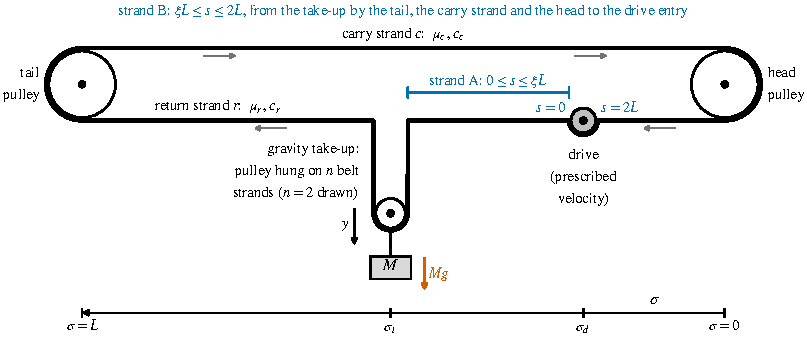
\includegraphics[width=\linewidth]{fig_loop}}{%
    \fbox{\parbox{0.9\linewidth}{\centering\vspace{3em}Loop schematic (run
    maps/fig\_loop.py).\vspace{3em}}}}
  \caption{Conveyor loop with the drive on the return strand. The geometric
  coordinate $\sigma$ runs from the head pulley along the return strand; the loop
  coordinate $s$ starts where the belt leaves the drive pulley ($s=0$) and ends where
  it returns to it ($s=2L$). The take-up at $s=\xi L$ divides the loop into strand~A,
  from the drive exit to the take-up, and strand~B, from the take-up by the tail, the
  carry strand and the head to the drive entry. Positions are illustrative.}
  \label{fig:loop}
\end{figure}

A geometric coordinate $\sigma\in[0,2L)$ is measured along the belt path in the
direction of travel, from the head pulley, so that the return strand occupies
$0\le\sigma<L$ and the carry strand $L\le\sigma<2L$; the tail pulley is at
$\sigma=L$ (\cref{fig:loop}). The drive pulley is at $\sigma_d$, anywhere on the
loop, and the take-up pulley at $\sigma_t\in(0,L)$, on the return strand. A head
drive corresponds to $\sigma_d=0$, a tail drive to $\sigma_d=L$ and an intermediate
drive to $0<\sigma_d<L$, with the take-up either downstream ($\sigma_t>\sigma_d$, on
the slack side) or upstream ($\sigma_t<\sigma_d$, on the tight side) of it.

The analysis uses the loop coordinate
\begin{equation}\label{eq:loopcoord}
  s=(\sigma-\sigma_d)\bmod 2L,\qquad s\in[0,2L],
\end{equation}
which starts where the belt leaves the drive pulley and ends where it returns to it;
$s=0$ and $s=2L$ are the two faces of the drive pulley. The take-up is at
$s_t=(\sigma_t-\sigma_d)\bmod 2L$, and $\xi=s_t/L$. In this coordinate the loop is an
open chain of homogeneous segments, separated by the head and tail pulleys, where the
line density changes, and by the take-up pulley. The take-up divides the chain into
strand~A ($0\le s\le s_t$) and strand~B ($s_t\le s\le 2L$). With a head drive,
strand~A is a piece of return belt of length $\xi L$, and strand~B holds the rest of
the return strand followed by the whole carry strand.

\subsection{Static state and dynamic increment}\label{sec:increment}

Let $\mw(s)$ be the line density that contributes to weight (belt and material,
without the reduced idler mass, so that $\mw\neq\mu$ in general), $\delta(s)$ the
local inclination of the belt path, positive uphill in the direction of travel, and
$\Tt$ the static belt tension at the take-up. At rest the static tension satisfies
\begin{equation}\label{eq:static}
  \frac{\dd T_0}{\dd s}=\mw(s)\,g\sin\delta(s),\qquad T_0(s_t)=\Tt,
\end{equation}
and the drive pulley, locked at rest, carries the difference $T_0(2L)-T_0(0)$. The
take-up holds $\Tt$ with the weight of its counterweight (Section~\ref{sec:static}).

During start-up the displacement of a belt particle is decomposed as
\begin{equation}\label{eq:decomposition}
  u(s,t)=u_0(s)+U(t)+w(s,t),\qquad U(t)=\int_0^tV(t')\,\dd t',
\end{equation}
where $u_0$ is the static displacement, $U$ the rigid-body motion imposed by the
drive and $w$ the elastic response. The rigid motion $U$ does not move the take-up,
because a uniform translation of the belt along its path leaves the length of belt
stored in the take-up unchanged. Balance of momentum of a belt element, after
subtraction of the static equilibrium~\eqref{eq:static}, gives in every segment
\begin{equation}\label{eq:pde}
  \mu(s)\,w_{tt}=\frac{\partial T_d}{\partial s}-\mu(s)\,a(t)-r(s)\,\varphi(t),
  \qquad T_d=EA\,(w_s+t_v\,w_{st}),
\end{equation}
with $a=\dot V$ the drive acceleration. The term $-\mu a$ is the inertial load of the
prescribed motion. The term $r(s)\varphi(t)$ represents the motion resistances
(idler rotation, indentation and flexure; force per unit length, opposing travel),
which are absent at rest and develop as the belt starts to move; $\varphi(t)$
describes their onset, with $\varphi\to1$ at steady speed. The base case is
$\varphi=V(t)/V_\infty$, with $V_\infty$ the final speed; a unit step serves as an
upper bound. A faithful representation would require resistances that depend on the
local belt speed, which is not attempted here.

Gravity does not appear in~\eqref{eq:pde}: it is balanced by the static state,
which includes the weight of the counterweight. Applying the weight as a load at
$t=0$ to a belt initially at rest and unstrained would excite a spurious transient of
the size of the static deflection. The simulations of \citet[Fig.~8]{lodewijks2013}
illustrate the superposition: during a drift stop of a \qty{1}{\kilo\metre} conveyor
whose path dips between head and tail, the dynamic drop of the carry-side tension in
the dip is the same, about \qty{17.3}{\kilo\newton}, for dips of
\qtyrange{0}{30}{\metre}, and the depth only shifts the static level. With a
\qty{40}{\metre} dip the tension drops to zero and the superposition fails, which is the slack limit of Section~\ref{sec:validity}. The
initial conditions are
\begin{equation}\label{eq:ic}
  w(s,0)=w_t(s,0)=0,\qquad y(0)=\dot y(0)=0,
\end{equation}
where $y$ is the displacement of the take-up pulley from its static position,
positive when the loop lengthens.

\subsection{Interface and boundary conditions}\label{sec:interfaces}

\paragraph{Drive pulley.} Without slip and with prescribed velocity, both faces of
the drive pulley follow $U(t)$; by~\eqref{eq:decomposition},
\begin{equation}\label{eq:bc_drive}
  w(0,t)=w(2L,t)=0.
\end{equation}

\paragraph{Head and tail pulleys.} By (A5) these pulleys transmit displacement and
tension unchanged,
\begin{equation}\label{eq:bc_ht}
  \jump{w}=0,\qquad \jump{T_d}=0,
\end{equation}
where $\jump{f}=f(s^+)-f(s^-)$. The same conditions hold at any other point where the
line density changes, such as the loading point.

\paragraph{Take-up pulley.} Consider first a pulley hung on the two belt branches
that wrap it by $180^\circ$ ($\nstr=2$). Because the pulley is free to rotate (A7),
the tension is the same on both sides,
\begin{equation}\label{eq:bc_tu_tension}
  T_d(s_t^-,t)=T_d(s_t^+,t)\equiv T_d(s_t,t).
\end{equation}
When the pulley moves by $y$, the belt stored around it grows by $2y$. In the loop
coordinate the take-up loop is collapsed to the point $s_t$, so the elongation of the
rest of the loop must grow by the same amount, $\int_0^{2L}w_s\,\dd s=2y$, the
integral being taken over the continuous parts. With~\eqref{eq:bc_drive},
\begin{equation}\label{eq:bc_tu_jump}
  \jump{w}_{s_t}=w(s_t^+,t)-w(s_t^-,t)=-2y(t):
\end{equation}
the belt upstream of the pulley is drawn forward into the take-up and the belt
downstream is drawn back. Finally, the two branches pull the pulley with $2T$; with
the static part balanced by the counterweight,
\begin{equation}\label{eq:bc_tu_dyn}
  \Mtu\,\ddot y=-2\,T_d(s_t,t).
\end{equation}
Equations~\eqref{eq:bc_tu_tension}--\eqref{eq:bc_tu_dyn} are the continuum
counterpart of the 2:1 take-up kinematics in the discrete models of
\citet[Eq.~7.55]{lodewijks1996} and \citet[Eqs.~4--5]{kulinowski2014}; in a continuum
model they were written by \citet[Eqs.~5--6]{song2012}, who then neglected the
take-up inertia. They follow from Hamilton's principle with kinetic energy
$\tfrac12\int\mu w_t^2\,\dd s+\tfrac12\Mtu\dot y^2$, strain energy
$\tfrac12\int EA\,w_s^2\,\dd s$ and the constraint~\eqref{eq:bc_tu_jump}: the
variation with respect to $w(s_t^\pm)$ gives~\eqref{eq:bc_tu_tension} and the
variation with respect to $y$ gives~\eqref{eq:bc_tu_dyn}. The static terms cancel
exactly, since the work of the static tension on the jump, $2\Tt y$, equals the work
of the take-up weight. The energy balance is
\begin{equation}\label{eq:energy}
  \frac{\dd}{\dd t}\left[\frac12\int_0^{2L}\!\left(\mu w_t^2+EA\,w_s^2\right)\dd s
  +\frac12\Mtu\dot y^2\right]
  =-\int_0^{2L}\!EA\,t_v\,w_{st}^2\,\dd s-\int_0^{2L}\!(\mu a+r\varphi)\,w_t\,\dd s .
\end{equation}

Eliminating $y$ between~\eqref{eq:bc_tu_jump} and~\eqref{eq:bc_tu_dyn} gives
$T_d(s_t)=(\Mtu/4)\,\jump{w_{tt}}_{s_t}$: the belt sees the take-up as a mass
$\Mtu/4$ in series, which resists only the relative acceleration of the two belt
ends and has no connection to the ground. This differs from a point mass embedded in
the belt (displacement continuous, tension jump $\jump{T_d}=\Mtu w_{tt}$), the
equivalent model of \citet[Fig.~2]{harrison1983} and the discrete model of
\citet{sakharwade2019}. The two models have opposite limits. As $\Mtu\to0$ the
embedded mass disappears, whereas the pulley enforces $T_d(s_t)=0$, a take-up of
constant force. As $\Mtu\to\infty$ the embedded mass becomes a fixed node, whereas
the pulley becomes a fixed pulley around which the belt runs freely and adds one slow
mode of the counterweight (Section~\ref{sec:properties}).

\subsection{Take-up hung on \texorpdfstring{$n$}{n} strands}\label{sec:nstrands}

Long conveyors often store belt in a multiple loop, with the carriage hung on
$\nstr$ belt strands ($\nstr$ even); $\nstr=4$ in the conveyor measured by
\citet{harrison1985b} and in the take-up described by \citet{nordell1997zisco}. With
carriage displacement $y_c$ and the same tension in all strands (free pulleys), the
conditions become $\jump{w}_{s_t}=-\nstr\,y_c$ and $\Mtu\ddot y_c=-\nstr\,T_d(s_t)$.
The equivalent displacement $y=(\nstr/2)\,y_c$ and the equivalent mass
\begin{equation}\label{eq:nmap}
  \Mtu_{\mathrm{eq}}=\frac{4\Mtu}{\nstr^2}
\end{equation}
recover~\eqref{eq:bc_tu_jump}--\eqref{eq:bc_tu_dyn} exactly and conserve the kinetic
energy, $\tfrac12\Mtu\dot y_c^2=\tfrac12\Mtu_{\mathrm{eq}}\dot y^2$. The static force on
the carriage is $\nstr\Tt$, the carriage travels $2/\nstr$ times the equivalent
displacement, and the length of belt stored, $2y$, does not depend on $\nstr$. The
number of take-up pulleys already enters the kinematics of the discrete model of
\citet{song2003}; here it only rescales the mass, and the rest of the paper is written
for the equivalent two-strand take-up. For the same take-up tension a multiple loop
reduces the equivalent mass by the factor $2/\nstr$ (Section~\ref{sec:static}), which
moves the take-up further towards the free-end regime of Section~\ref{sec:freeend}.

\subsection{Take-up mass and static tension}\label{sec:static}

The take-up mass is not a free parameter. Let $M_w$ be the counterweight mass, $M_c$
the mass of the take-up pulley and carriage, $\lambda$ the rigging ratio
(counterweight travel per unit carriage travel; $\lambda=1$ for a counterweight hung
directly on the carriage) and $\delta_c$ the inclination of the carriage track
($\delta_c=90^\circ$ for a vertical take-up). Virtual work and kinetic energy give
\begin{equation}\label{eq:reeving}
  \nstr\,\Tt=g\,(\lambda M_w+M_c\sin\delta_c),\qquad
  \Mtu=M_c+\lambda^2M_w=\frac{\lambda\,\nstr\,\Tt}{g}+(1-\lambda\sin\delta_c)\,M_c .
\end{equation}
With the equivalent mass~\eqref{eq:nmap} and the weight of the return strand
$\Wr=g\mu_rL$, the take-up mass ratio defined in Section~\ref{sec:dimensionless}
becomes
\begin{equation}\label{eq:beta_tension}
  \beta=\frac{4\Mtu}{\nstr^2\mu_rL}
  =\frac{4}{\nstr}\,\lambda\,\frac{\Tt}{\Wr}+\frac{4(1-\lambda\sin\delta_c)\,M_c}{\nstr^2\mu_rL}.
\end{equation}
The second term vanishes for a vertical take-up with a directly hung counterweight
and is otherwise small, since the carriage weighs much less than the counterweight.
Equation~\eqref{eq:beta_tension} states that the take-up mass follows from the
take-up tension: rigging and multiple loops change the mass for a given tension, but
a gravity take-up cannot combine a large tension with a small mass. The tension $\Tt$
is fixed by the running-state design: it is the smallest value that satisfies the
grip condition at the drive and the sag limits on both strands, plus whatever margin
the designer adds. It therefore depends weakly on the take-up position; for a
horizontal head-drive conveyor governed by grip, for example,
$\Tt=T_{2,\min}+r_r\,\xi L$, where $T_{2,\min}$ is the least admissible slack-side
tension and $r_r$ the running resistance per unit length of the return strand.
Section~\ref{sec:masscorrection} shows that the mass enters the dynamics only as a
correction, which is why the results are given in terms of $\xi$ and $\gamma$ with
$\beta$ as a correction; Section~\ref{sec:betaregime} evaluates $\Tt/\Wr$ for the
conveyors in the literature.

\subsection{Dimensionless formulation}\label{sec:dimensionless}

Lengths are scaled by $L$, times by the transit time of the return strand $L/c_r$,
accelerations by the peak drive acceleration $a_m$, displacements by $a_mL^2/c_r^2$
and tensions by the inertial force of the return strand $\mu_rLa_m$:
\begin{equation}\label{eq:scales}
  x=\frac{s}{L},\quad \tau=\frac{c_rt}{L},\quad
  \hat w=\frac{c_r^2}{a_mL^2}\,w,\quad \hat y=\frac{c_r^2}{a_mL^2}\,y,\quad
  \hat T=\frac{T_d}{\mu_rLa_m},\quad \hat a=\frac{a}{a_m},\quad
  \hat r=\frac{r}{\mu_ra_m}.
\end{equation}
The dimensionless parameters are
\begin{equation}\label{eq:params}
  \gamma=\frac{c_r}{c_c}=\sqrt{\frac{\mu_c}{\mu_r}},\qquad
  \beta=\frac{4\Mtu}{\nstr^2\mu_rL},\qquad
  \xi=\frac{s_t}{L},\qquad
  \hat\zeta=\frac{c_rt_v}{2L},\qquad
  \tau_a=\frac{c_rt_a}{L},
\end{equation}
together with the drive position $\sigma_d/L$ and the shape of the start-up profile,
whose acceleration time is $t_a$. For $\nstr=2$, $\beta=\Mtu/(\mu_rL)$. The relative
line density is $\hat\mu(x)=1$ on the return strand and $\gamma^2$ on the carry
strand. Since $EA=\mu_rc_r^2$, the problem~\eqref{eq:pde}--\eqref{eq:bc_tu_dyn}
becomes
\begin{gather}
  \hat\mu\,\hat w_{\tau\tau}=\frac{\partial\hat T}{\partial x}-\hat\mu\,\hat a(\tau)
  -\hat r(x)\,\varphi(\tau),\qquad \hat T=\hat w_x+2\hat\zeta\,\hat w_{x\tau},\label{eq:pde_nd}\\
  \hat w(0,\tau)=\hat w(2,\tau)=0,\qquad \jump{\hat w}_\xi=-2\hat y,\qquad
  \jump{\hat T}_\xi=0,\qquad \beta\,\hat y_{\tau\tau}=-2\,\hat T(\xi,\tau),\label{eq:bc_nd}
\end{gather}
with $\hat w$ and $\hat T$ continuous at the head and tail pulleys. In the elastic case
the dimensionless dynamic tension equals the dimensionless strain.

% =====================================================================
% Section 3 -- Closed-form solution. Written in step 6.3 from model.tex
% with notes 4.3, 4.4, 4.6, 4.9 points 1-3, 6 and 11, 4.10 and 4.14.
% Decision of step 6.3: the torque-controlled drive stays here (3.6),
% because Section 4 uses m_d and the slip dashpot for Harrison's case.
% Every formula is checked in beltloop/tests (see the comments).
% =====================================================================
\section{Closed-form solution}\label{sec:solution}

\subsection{Transfer matrices and characteristic equation}\label{sec:eigen}

Undamped free vibration, $\hat w=W(x)\,\ee^{\ii\Omega\tau}$ and
$\hat y=Y\ee^{\ii\Omega\tau}$, with dimensionless frequency $\Omega=\omega L/c_r$,
gives
\begin{equation}\label{eq:eigen}
  W''+\kappa_j^2W=0\ \text{in segment } j,\qquad \kappa_r=\Omega,\quad \kappa_c=\gamma\Omega,
\end{equation}
with $W(0)=W(2)=0$, $W$ and $W'$ continuous at the head and tail pulleys, and, at the
take-up,
\begin{equation}\label{eq:eigen_tu}
  \jump{W'}_\xi=0,\qquad Y=\frac{2\,W'(\xi)}{\beta\Omega^2},\qquad
  \jump{W}_\xi=-\frac{4\,W'(\xi)}{\beta\Omega^2}.
\end{equation}
With the state vector $\mat z=(W,W')^\T$, a homogeneous segment of length $\ell$ and
wavenumber $\kappa$, and the take-up pulley, act through the unimodular matrices
\begin{equation}\label{eq:transfer}
  \mat S(\ell,\kappa)=\begin{pmatrix}\cos\kappa\ell&\kappa^{-1}\sin\kappa\ell\\
  -\kappa\sin\kappa\ell&\cos\kappa\ell\end{pmatrix},\qquad
  \mat J=\begin{pmatrix}1&-4/(\beta\Omega^2)\\0&1\end{pmatrix}.
\end{equation}
Let $\mat A(\Omega)$ be the product of the segment matrices of strand~A, from the
drive exit to the take-up, and $\mat B(\Omega)$ that of strand~B, from the take-up to
the drive entry, so that $\mat z(2)=\mat B\mat J\mat A\,\mat z(0)$ with
$\mat z(0)=(0,1)^\T$. The condition $W(2)=0$ and the identity
$(\mat B\mat J\mat A)_{12}=(\mat B\mat A)_{12}-4A_{22}B_{11}/(\beta\Omega^2)$ give the
characteristic equation
\begin{equation}\label{eq:chareq}
  D(\Omega)\equiv\beta\,\Omega^2\,(\mat B\mat A)_{12}-4\,A_{22}\,B_{11}=0 .
\end{equation}
$D$ is an entire function of $\Omega$, so its zeros can be bracketed without
spurious roots at poles, and $D(0)=-4$: with the velocity prescribed at the drive
there is no rigid-body mode. Each term has a direct meaning. $(\mat B\mat A)_{12}=0$
gives the modes of the loop with the take-up pulley fixed in space (the belt fixed at
both faces of the drive and running freely around the take-up pulley); $A_{22}=0$
gives the modes of strand~A fixed at the drive and free of dynamic tension at the
take-up, and $B_{11}=0$ the same for strand~B. \Cref{app:transfer} lists $\mat A$
and $\mat B$ for every position of the drive; with at most three factors in each
product, $D$ is an explicit trigonometric polynomial in $\Omega$ and $\gamma\Omega$.
For a head drive ($\sigma_d=0$, $\xi=\sigma_t/L$),
\begin{equation}\label{eq:chareq_head}
  \begin{split}
  \gamma\,D(\Omega)={}&\beta\Omega\left[\gamma\sin\Omega\cos\gamma\Omega+\cos\Omega\sin\gamma\Omega\right]\\
  &-4\cos\Omega\xi\left[\gamma\cos\Omega(1-\xi)\cos\gamma\Omega-\sin\Omega(1-\xi)\sin\gamma\Omega\right].
  \end{split}
\end{equation}
The mode shapes follow by propagating $\mat z(0)=(0,1)^\T$ through the chain.
% tests: test_eigen.py (D against independent FE); verify_phase2 checks in test_modes.py

\subsection{Properties}\label{sec:properties}

\begin{enumerate}
  \item \emph{Direction of travel.} Reversing the direction of travel reverses the
  chain and leaves~\eqref{eq:chareq} unchanged (\cref{app:transfer}); the spectrum is
  a property of the loop, consistent with (A4).
  \item \emph{Uniform loop} ($\gamma=1$). Since $(\mat B\mat A)_{12}=\sin2\Omega/\Omega$,
  $A_{22}=\cos\Omega\xi$ and $B_{11}=\cos\Omega(2-\xi)$,
  \begin{equation}\label{eq:chareq_uniform}
    \tan\Omega\xi+\tan\Omega(2-\xi)=\frac{4}{\beta\Omega}:
  \end{equation}
  only the distance from the drive to the take-up along the loop matters, and the
  equation is symmetric under $\xi\to2-\xi$. The embedded-mass model of
  Section~\ref{sec:interfaces} gives instead $\cot\Omega\xi+\cot\Omega(2-\xi)=\beta\Omega$.
  \item \emph{Heavy take-up} ($\beta\to\infty$). The roots tend to those of
  $(\mat B\mat A)_{12}=0$, plus one slow mode, $\Omega_0\simeq\sqrt{2/\beta}$, in which
  the counterweight oscillates against the stiffness of the loop. Rayleigh's quotient
  with the quasi-static shape ($W=x$ upstream and $W=x-2$ downstream of the take-up,
  for $Y=1$) gives the bound
  \begin{equation}\label{eq:rayleigh}
    \Omega_0^2\le\frac{2}{\beta+\beta_b},\qquad \beta_b=\int_0^2\hat\mu\,W^2\,\dd x,
  \end{equation}
  with $\beta_b=[\xi^3+(2-\xi)^3]/3$ for $\gamma=1$. The bound is useful only for
  $\beta\gg\beta_b$, which is not the regime of long conveyors
  (Section~\ref{sec:betaregime}).
  \item \emph{Take-up at the tail} ($\gamma=1$, $\xi=1$). Equation~\eqref{eq:chareq_uniform}
  factorises into $\cos\Omega=0$, modes with zero dynamic tension at the take-up,
  which stays at rest, and $\Omega\tan\Omega=2/\beta$, modes in which the take-up
  moves. The second family is the characteristic equation $\eta\tan\eta=\alpha_{LP}$,
  $\alpha_{LP}=2\mu_rL/\Mtu$, used by \citet{li2018} for a tail take-up and by
  \citet{pang2015} for a single span with a mass at its end: each strand carries half
  of the take-up inertia, because both strand ends move by $y$. The embedded-mass
  model shares this family and replaces the first by $\sin\Omega=0$. The case checks
  the formulation but does not discriminate between take-up models. Moreover, the
  drive acceleration excites only the first family, whose modes leave the take-up at
  rest: in this configuration the response to the drive acceleration does not depend
  on the take-up mass (Section~\ref{sec:frequencies}).
  \item \emph{Interlacing.} Dividing~\eqref{eq:chareq} by $\beta\Omega^2A_{22}B_{11}$
  gives
  \begin{equation}\label{eq:receptance}
    H_A(\Omega)+H_B(\Omega)=\frac{4}{\beta\Omega^2},\qquad
    H_A=\frac{A_{12}}{A_{22}},\quad H_B=\frac{B_{12}}{B_{11}},
  \end{equation}
  where $H_A$ and $H_B$ are the receptances of strands A and B at their free ends:
  the displacement of the strand end per unit dynamic tension, with the strand fixed
  at the drive. By Green's identity each receptance increases with $\Omega$ between
  its poles, which are the fixed--free frequencies of the strand, whereas the
  right-hand side decreases. Hence the natural frequencies interlace strictly with
  the union of the fixed--free frequencies of the two strands: there is exactly one
  root below the lowest strand frequency and exactly one between consecutive strand
  frequencies, and a pair of coincident strand frequencies is itself a root. Every
  mode of the loop therefore lies between two modes of the strands with the take-up
  free. For small $\beta$, pairs of roots close to nearly coincident strand
  frequencies are separated by $O(\beta)$ and are easily missed by a grid search;
  bracketing the roots between consecutive strand frequencies finds all of them
  (\cref{app:numerics}).
  % tests: test_eigen.py (interlacing, all roots), test_beta_regime.py (Li-Pang tail)
\end{enumerate}

\subsection{The take-up as a free end}\label{sec:freeend}

As $\beta\to0$, Eq.~\eqref{eq:chareq} reduces to $A_{22}B_{11}=0$, and the take-up
condition~\eqref{eq:bc_nd} to $\hat T(\xi,\tau)=0$ at all times: a light take-up is a
device of constant force. The loop then splits into strands A and B, each fixed at
the drive and free at the take-up, whose lengths are set by the take-up position. The
split holds for the forced response as well, since a free end transmits no force:
during a start-up each strand responds to its own inertial and resistance loads, and
the take-up moves by half the sum of the elongations of the two strands. For a head
drive, the frequencies of strand~B follow from
\begin{equation}\label{eq:strandB}
  \tan\Omega(1-\xi)\,\tan\gamma\Omega=\gamma,
\end{equation}
and those of strand~A, a uniform piece of return belt, are $(2j-1)\pi/(2\xi)$. For
$\gamma=1$ the fundamental is the quarter-wave mode of the longer strand,
$\Omega_1=\pi/[2(2-\xi)]$ for $\xi<1$; with the take-up next to the drive its period
is $8L/c_r$, twice that with the take-up at the tail. Section~\ref{sec:frequencies}
develops the consequences: the fundamental belongs to the strand that contains the
carry strand, and moving the take-up changes the spectrum.

The free-end limit also governs wave propagation. A harmonic wave on the return
strand that meets the take-up is transmitted with the complex coefficient
\begin{equation}\label{eq:transmission}
  \chi=\frac{1}{1-2\ii/(\beta\Omega)},\qquad
  |\chi|=\frac{\beta\Omega}{\sqrt{\beta^2\Omega^2+4}}=\frac{\Mtu_{\mathrm{eq}}\,\omega}
  {\sqrt{\Mtu_{\mathrm{eq}}^2\omega^2+4Z_r^2}},
\end{equation}
obtained from $\mat J$ with an incident and a reflected wave on one side and a
transmitted wave on the other; $Z_r=\mu_rc_r$ is the impedance of the return strand
and $|\chi|^2+|1-\chi|^2=1$. The take-up is opaque, $|\chi|\to0$, when its inertial
impedance is small against twice that of the belt, $\Mtu_{\mathrm{eq}}\,\omega\ll2Z_r$,
and transparent, $|\chi|\to1$, in the opposite limit. In a long conveyor the
stretching front of a start-up is therefore reflected at the take-up as at a free
end, and the return belt beyond it stays at rest until the front arrives the other
way round the loop. This is the mechanism recorded by \citet{harrison1985b}, which
Section~\ref{sec:validation} compares with the model. An embedded mass behaves in the
opposite way: it becomes transparent as its mass decreases.
% tests: test_harrison.py::test_takeup_transmission_from_J (energy, both limits)

\subsection{Closed-form correction for the take-up mass}\label{sec:masscorrection}

For finite $\beta$ the receptance form~\eqref{eq:receptance} gives a closed-form
correction. Each receptance is a sum over the fixed--free modes of its strand,
\begin{equation}\label{eq:receptance_sum}
  H_s(\Omega)=\sum_j\frac{1}{\tilde m_{s,j}\,(\Omega_{s,j}^2-\Omega^2)},\qquad s\in\{A,B\},
\end{equation}
where $\Omega_{s,j}$ are the fixed--free frequencies and $\tilde m_{s,j}=m_{s,j}/W_{s,j}(\xi)^2$
the modal mass seen from the free end; for a uniform strand of length $\ell$ and
density $\hat\mu$, $\tilde m=\hat\mu\ell/2$ for every mode. Keeping a single pole
$\Omega_p$ of modal mass $\tilde m$,
\begin{equation}\label{eq:onepole}
  \Omega\simeq\frac{\Omega_p}{\sqrt{1+\beta/(4\tilde m)}},
\end{equation}
which is Rayleigh's quotient of the fixed--free mode with a mass $\beta/4$ attached to
its free end. In physical terms, the take-up mass $\Mtu_{\mathrm{eq}}/4$ is a tip mass
on the strand, and for a uniform strand the period lengthens by about
$(\Mtu_{\mathrm{eq}}/4)/m_s$, with $m_s$ the mass of the strand. When a frequency of
the other strand is close, both poles are kept: with $u=\Omega^2$, $P_s=\Omega_{p,s}^2$
and $b_s=1/\tilde m_s$,
\begin{equation}\label{eq:twopole}
  \bigl[4+\beta(b_A+b_B)\bigr]u^2-\bigl[4(P_A+P_B)+\beta(b_AP_B+b_BP_A)\bigr]u+4P_AP_B=0 .
\end{equation}
For coincident poles one root stays at the pole and the other shifts with both
strands, as in the family $\Omega\tan\Omega=2/\beta$ of the tail take-up
(Section~\ref{sec:properties}). Against the exact roots, for a head drive,
$1\le\gamma\le3$ and the take-up anywhere on the return strand, the frequencies
of~\eqref{eq:twopole} are within \qty{\NumMassCorrErrTenth}{\percent} for
$\beta\le0.1$ (first three modes) and the fundamental within
\qty{\NumMassCorrErrFundOne}{\percent} up to $\beta=1$. Higher modes deviate for
$\beta\sim1$, where the slow mode of the counterweight, $\Omega_0\simeq\sqrt{2/\beta}$,
enters the spectrum of the belt.

The take-up mass is thus a correction to the free-end spectrum, of relative size
$\beta/(8\tilde m)$ on each frequency. The results of Section~\ref{sec:results} are
computed with the exact roots, but organised around the free-end limit, with the
mass as a correction whose size is mapped in Section~\ref{sec:betaregime}.
% tests: test_beta_regime.py (m_tilde = l/2, residues, single and two poles, accuracy);
% numbers: paper_numbers.py, section "Closed-form solution"

\subsection{Modal expansion and start-up response}\label{sec:modal}

The modes are orthogonal with respect to the inner product
\begin{equation}\label{eq:inner}
  \bigl\langle(W_i,Y_i),(W_j,Y_j)\bigr\rangle=\int_0^2\hat\mu\,W_iW_j\,\dd x+\beta\,Y_iY_j,
\end{equation}
and $\int_0^2W_i'W_j'\,\dd x=\Omega_i^2\,m_i\,\delta_{ij}$, with modal mass
$m_i=\langle(W_i,Y_i),(W_i,Y_i)\rangle$ (\cref{app:transfer}). Both the density
weight and the take-up term are required; the unweighted product does not
diagonalise the problem. The Kelvin--Voigt term acts only through the belt strain,
and neither the take-up nor the drive adds stiffness, so damping is proportional to
stiffness and the modes stay uncoupled. With $\hat w=\sum_kp_k(\tau)W_k(x)$ and
$\hat y=\sum_kp_k(\tau)Y_k$, the weak form of~\eqref{eq:pde_nd}--\eqref{eq:bc_nd} gives
\begin{equation}\label{eq:modal}
  p_k''+2\zeta_k\Omega_k\,p_k'+\Omega_k^2\,p_k=-\Gamma_k\,\hat a(\tau)-R_k\,\varphi(\tau),
  \qquad p_k(0)=p_k'(0)=0,
\end{equation}
with
\begin{equation}\label{eq:participation}
  \zeta_k=\hat\zeta\,\Omega_k=\frac{t_v\,\omega_k}{2},\qquad
  \Gamma_k=\frac{1}{m_k}\int_0^2\hat\mu\,W_k\,\dd x,\qquad
  R_k=\frac{1}{m_k}\int_0^2\hat r\,W_k\,\dd x .
\end{equation}
The damping ratio grows linearly with frequency, as in the formulation of
\citet{pihnastyi2020}. The inertial load has no component on the take-up, because the
rigid motion $U$ does not move it; for this reason $\Gamma_k$ has no $\beta Y_k$ term.
By completeness of the modes in the space weighted by~\eqref{eq:inner}, the effective
modal masses add up to the mass of the belt,
\begin{equation}\label{eq:parseval}
  \sum_k\Gamma_k^2\,m_k=\int_0^2\hat\mu\,\dd x=1+\gamma^2,
\end{equation}
so $\Gamma_k^2m_k/(1+\gamma^2)$ is the fraction of the belt inertia excited by the
start-up in mode $k$. The dynamic tension and the take-up displacement are
\begin{equation}\label{eq:outputs}
  \hat T(x,\tau)=\sum_k\left(p_k+2\hat\zeta\,p_k'\right)W_k'(x),\qquad
  \hat y(\tau)=\sum_kp_k\,Y_k .
\end{equation}

\paragraph{Quasi-static limit.} When the loads vary slowly compared with the
fundamental period, $p_k\simeq-(\Gamma_k\hat a+R_k\varphi)/\Omega_k^2$ and the series
sums to
\begin{equation}\label{eq:quasistatic}
  \hat T_{\mathrm{qs}}(x,\tau)=\hat a(\tau)\int_\xi^x\hat\mu\,\dd x'
  +\varphi(\tau)\int_\xi^x\hat r\,\dd x',\qquad
  \hat y_{\mathrm{qs}}(\tau)=\frac12\int_0^2\hat T_{\mathrm{qs}}\,\dd x .
\end{equation}
The take-up anchors the dynamic tension at zero, and the loads accumulate from the
take-up towards the drive in both directions: the tension rises from the take-up to
the drive entry and falls from the take-up back to the drive exit. The quasi-static
field does not depend on $\beta$, nor on the damping: without inertia a Kelvin--Voigt
belt carries exactly the applied tension, and only its strain lags, with the time
constant $t_v$, equally in every mode. The take-up displacement is half the
elongation of the loop; for a head drive and inertial load alone,
$\hat y_{\mathrm{qs}}=\tfrac12\bigl(\tfrac32-2\xi+\tfrac12\gamma^2\bigr)\hat a$.
Equation~\eqref{eq:quasistatic} is the reference for the dynamic amplification
factors of Section~\ref{sec:startup}.

\paragraph{Start-up profiles.} The base case is the sinusoidal acceleration
\begin{equation}\label{eq:profile}
  a(t)=a_m\sin\frac{\pi t}{t_a}\quad(0\le t\le t_a),\qquad a_m=\frac{\pi V_\infty}{2t_a},
\end{equation}
with $a=0$ for $t>t_a$; triangular and parabolic acceleration profiles serve for
comparison. In dimensionless form $\hat a=\sin\varpi\tau$ on $0\le\tau\le\tau_a$, with
$\varpi=\pi/\tau_a$. The modal equations~\eqref{eq:modal} are integrated exactly for
any piecewise-polynomial profile and onset (\cref{app:numerics}). Without damping,
the free oscillation that the acceleration phase leaves in mode $k$ has amplitude
\begin{equation}\label{eq:residual}
  P_k=\frac{|\Gamma_k|}{\Omega_k}\left|\int_0^{\tau_a}\hat a(\tau')\,
  \ee^{\ii\Omega_k\tau'}\dd\tau'\right|
  =\frac{|\Gamma_k|}{\Omega_k}\,\frac{2\varpi\,|\cos(\Omega_k\tau_a/2)|}{|\varpi^2-\Omega_k^2|},
\end{equation}
with the limit $|\Gamma_k|\tau_a/(2\Omega_k)$ at $\Omega_k=\varpi$, and a residual
tension $P_k|W_k'(x)|$. This is the classical residual spectrum of a half-sine pulse:
it vanishes when $t_a=(j+\tfrac12)\,t_k$, $j=1,2,\dots$, where $t_k=2\pi/\omega_k$ is the
modal period, and decays as $\Omega_k^{-3}$ for $\Omega_k\gg\varpi$.

\paragraph{Motion resistances.} With a unit step $\varphi$, each mode overshoots its
quasi-static response by a factor of two, but the tension field is not bounded by
that factor: with $\gamma=2$, $\beta=0.1$ and $\xi=0.05$, the undamped peak at the
drive entry reaches \NumStepOvershootEntry\ times the quasi-static value. The factor
is two only for a uniform loop with a light take-up. A smooth onset,
$\varphi=V/V_\infty$, removes most of the overshoot (Section~\ref{sec:startup}).
% tests: test_response.py::test_step_overshoot_can_exceed_two (2.18, confirmed with FE)

\paragraph{Admissibility.} The linear solution holds while three conditions are met
(Section~\ref{sec:validity}). (i)~The total tension, static tension at rest plus
dynamic tension with the resistances included, stays positive along the loop; in
steady running this sum is the running tension. (ii)~The take-up follows the belt:
the total tension at the take-up stays positive, $\ddot y_c<\nstr\Tt/\Mtu$, which for a
counterweight hung directly ($\lambda=1$, carriage mass neglected) reads $\ddot y_c<g$:
the counterweight cannot be required to fall faster than gravity. (iii)~The drive
does not slip, $T(2L,t)\le\egrip\,T(0,t)$ throughout the start, where $T$ is the total
tension at the drive entry and exit.

\subsection{Limit of validity: drive without speed control}\label{sec:torque}

If the drive imposes a torque instead of a velocity, its faces move with an unknown
displacement and the drive acts as a mass $M_d=J_d/R_d^2$ that joins the two ends of
the loop ($J_d$ is the drive inertia reduced to the pulley shaft and $R_d$ the pulley
radius). The linearised slip of an induction motor adds a viscous force towards the
reference speed, with coefficient $c_d$. With $m_d=M_d/(\mu_rL)$ and
$\hat c=c_d/(\mu_rc_r)$, the drive conditions become $W(0)=W(2)$ and
$W'(0)-W'(2)=-(m_d\Omega^2-\ii\hat c\,\Omega)\,W(0)$, and the characteristic equation is
\begin{equation}\label{eq:chareq_torque}
  2-\operatorname{tr}\mat P+\left(m_d\Omega^2-\ii\hat c\,\Omega\right)P_{12}=0,
  \qquad \mat P=\mat B\mat J\mat A,
\end{equation}
whose roots are complex when $\hat c>0$ (with the convention $\ee^{\ii\Omega\tau}$,
damped roots have $\operatorname{Im}\Omega>0$). For $m_d\to\infty$ or $\hat c\to\infty$
it reduces to $P_{12}=0$, the prescribed velocity~\eqref{eq:chareq}. For $m_d\to0$
and $\hat c=0$ it gives the periodic condition $\operatorname{tr}\mat P=2$ of a free loop,
which has a rigid-body mode: with the take-up next to the drive, $\beta\to0$ and
$\gamma=1$, the fundamental changes from the quarter-wave mode of the loop under
prescribed velocity (period $8L/c_r$) to its half-wave mode (period $4L/c_r$). With
$m_d=0$ and $\beta\to0$ the dashpot alone reflects waves at the drive with the real
coefficient $(\hat c-1)/(\hat c+1)$; for $\hat c>1$ it leaves the period of the
prescribed-velocity limit unchanged and only adds damping, with
$\operatorname{Re}\Omega=\pi/[2(2-\xi)]$ and
$\operatorname{Im}\Omega=\ln\bigl[(\hat c+1)/(\hat c-1)\bigr]/[2(2-\xi)]$ for $\gamma=1$
as $\xi\to0$. The prescribed velocity therefore represents drives whose speed is
controlled in closed loop, as recommended for start-up and stopping of long
conveyors \citep{jennings2013} and as in the frequency-controlled starts of
\citet[\S8.6.2]{lodewijks1996}, or whose reduced inertia is large compared with the
mass of the belt. Section~\ref{sec:validation} uses Eq.~\eqref{eq:chareq_torque} to
test this assumption on a conveyor with a wound-rotor drive.
% tests: test_harrison.py::test_damped_drive_limits; test_eigen.py (torque variant vs FE)

% =====================================================================
% Section 4 -- Verification and validation, in three levels. Step 6.4.
% Inputs: claims 3(a)-(d) in section 3 of the notes; validation figure
% and caption (notes 4.9, end); notes 4.10, 4.11, 4.13; 4.9 points 5, 7, 10.
% =====================================================================
\section{Verification and validation}\label{sec:validation}

\subsection{Verification against an independent lumped-mass model}\label{sec:lumped}
\begin{figure}[t]
  \centering
  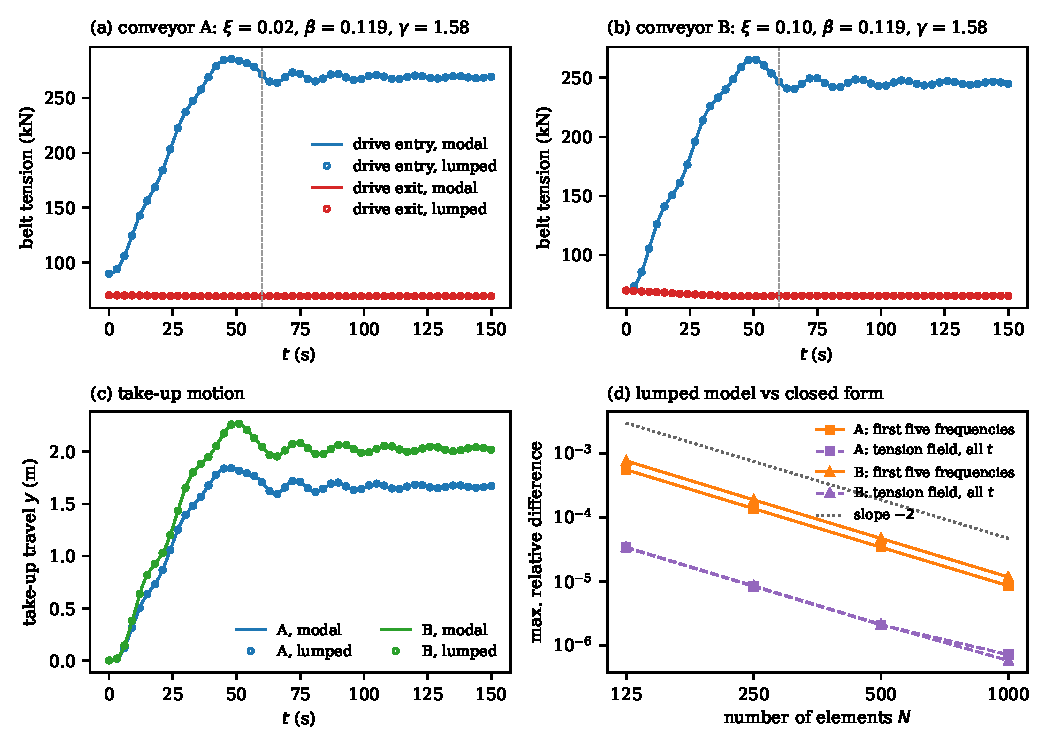
\includegraphics[width=\linewidth]{lumped_validation}
  \caption{\TODO{Validation caption (notes 4.9, end).}}
  \label{fig:validation}
\end{figure}
\TODO{Lumped-mass verification.}

\subsection{Consistency with field records}\label{sec:fieldchecks}
% Harrison (1983, 1985b): slow period 25 s, compatible only with a nearly
% free take-up and a speed-rigid drive (consistency check, not a proof).
% Kinematic checks: nordell1984 (wave arrival), Muja (cdi1998: 3.1 s over
% 6.1 km). Declare what the model does not reproduce (notes 4.10).
\TODO{Consistency checks.}

\subsection{Cross-comparison with other models}\label{sec:crosscheck}
% lodewijks1996 ch. 8 (peaks agree, dynamics do not; notes 4.11) and
% song2012 (notes 4.12).
\TODO{Cross-comparison.}

% =====================================================================
% Section 5 -- Results. Steps 6.5 (5.1-5.2) and 6.6 (5.3-5.4).
% Inputs: notes 4.15-4.19 and 4.26; 4.9 points 13, 14, 16-18;
% captions.md (draft captions, to be moved into the .tex in 6.5-6.6).
% Mechanics first (JSV emphasis); engineering material condensed.
% =====================================================================
\section{Results}\label{sec:results}

\subsection{Natural frequencies and modal participation}\label{sec:frequencies}
\begin{figure}[t]
  \centering
  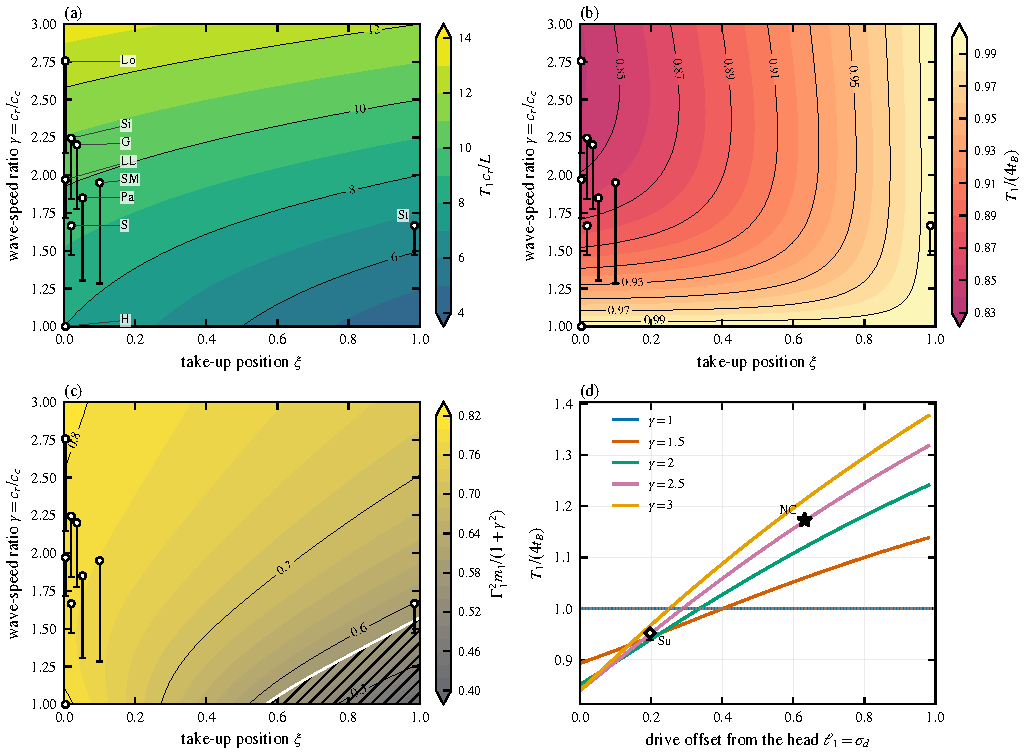
\includegraphics[width=\linewidth]{fig_modal}
  \caption{\TODO{fig\_modal caption (captions.md).}}
  \label{fig:modal}
\end{figure}
% Modes followed by strand; the fundamental belongs to strand B (Rayleigh)
% with bounds 4 gamma < tau_1 <= 4 tau_B; formula for F_1; intermediate drive.
\TODO{Frequencies and participation by strand; intermediate drive.}

\subsection{When the take-up mass matters}\label{sec:betaregime}
\begin{figure}[t]
  \centering
  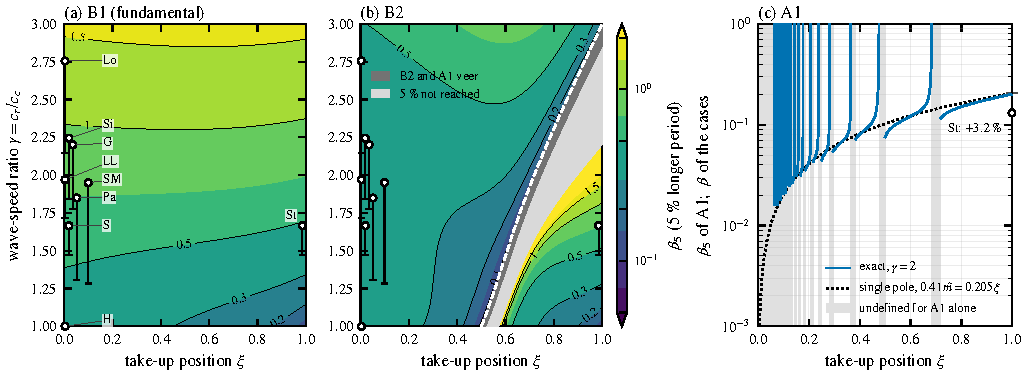
\includegraphics[width=\linewidth]{fig_beta}
  \caption{\TODO{fig\_beta caption (captions.md).}}
  \label{fig:beta}
\end{figure}
% Generated by maps/paper_tables.py (phase 5.6) from maps/cases.py; do not edit by hand.
\begin{table*}[t]
\centering
\footnotesize
\setlength{\tabcolsep}{3.0pt}
\begin{threeparttable}
\caption{Conveyors from the literature, by decreasing length. $\xi$: take-up position from the drive exit along the return strand, in units of $L$; $\mu_r$: inertial line density of the return strand (belt and reduced idler mass); $\gamma=c_r/c_c$ at full material coupling ($\alpha=1$) and, in brackets, at the lowest coupling of the material class \citep{lodewijks2002}; $c_r$: wave speed of the return strand; $T_1$: fundamental period with the take-up mass ($\alpha=1$); $T_t$: static belt tension at the take-up; $n$: belt strands that carry the take-up pulley; $W_r=g\mu_rL$; $\beta=4M/(n^2\mu_rL)=(4/n)\lambda T_t/W_r$; $\beta_5$: take-up mass that lengthens the fundamental by 5\,\% at the case's $\xi$ and $\gamma$. Last column: what set $T_t$ according to the source.}
\label{tab:cases}
\begin{tabular}{@{}lrcrlrrrclll>{\raggedright\arraybackslash}p{24mm}@{}}
\toprule
Case & $L$ & $\xi$ & $\mu_r$ & $\gamma$ & $c_r$ & $T_1$ & $T_t$ & $n$ & $T_t/W_r$ & $\beta$ & $\beta/\beta_5$ & $T_t$ set by \\
 & (km) & & (kg/m) & & (m/s) & (s) & (kN) & & & & & \\
\midrule
Si & 13.10 & 0.001 & 35.3$^{\mathrm{c}}$ & 2.24$^{\mathrm{c}}$ (1.84) & 2171$^{\mathrm{c}}$ & 66.1$^{\mathrm{c}}$ & 115.0 & 2 & 0.025$^{\mathrm{c}}$ & 0.025$^{\mathrm{c}}$ & 0.03$^{\mathrm{c}}$ & full-load braking \\
LL & 7.60 & 0.005 & 66.9 & 1.97 (1.72) & 1649 & 46.8$^{\mathrm{a}}$ & 209.9$^{\mathrm{a}}$ & 2$^{\mathrm{a}}$ & 0.042$^{\mathrm{a}}$ & 0.084$^{\mathrm{a}}$ & 0.11$^{\mathrm{a}}$ & start grip (checked) \\
S & 7.12 & 0.001 / 0.999 & 37.8 & 1.67 (1.47) & 1659 & 40.4 / 29.0 & 173.0 & 2 & 0.066 & 0.131 & 0.22 / 0.27 & not stated (grip at $E = 2.98$) \\
H & 5.10 & 0.005 & 81.4 & 0.97$^{\mathrm{m}}$ & 1428$^{\mathrm{m}}$ & 28.4 & 49.0 & 4 & 0.012 & 0.012 & 0.03 & not stated (grip at $E \ge 4.1$) \\
G & 4.50 & 0.001 & 40.1 & 2.20 (1.77) & 1972 & 24.6$^{\mathrm{a}}$ & -- & -- & -- & 0.006$^{\mathrm{a}}$ & 0.01$^{\mathrm{a}}$ & unknown \\
SM & 3.00 & 0.100 & 72.7 & 1.95 (1.28) & 2181$^{\mathrm{c}}$ & 13.6$^{\mathrm{a}}$ & 140.0 & 2$^{\mathrm{a}}$ & 0.065 & 0.131$^{\mathrm{a}}$ & 0.17$^{\mathrm{a}}$ & not stated (model input) \\
Pa & 2.56 & 0.020 & 138.0 & 1.85 (1.30) & 2665 & 9.5 & 292.0 & 2 & 0.084 & 0.169 & 0.24 & not stated (about 2\,\% sag) \\
NC & 2.48 & 0.037 & -- & 2.46 & 1450 & 27.5 & -- & -- & -- & -- & -- & unknown \\
Lo & 1.00 & 0.001 & 21.2 & 2.76 (2.15) & 446 & 28.5 & 21.3 & 2 & 0.102 & 0.205 & 0.15 & start grip (sized) \\
Su & 0.81 & 0.010 & 39.9 & 2.58 (2.01) & 1840$^{\mathrm{c}}$ & 6.1$^{\mathrm{c}}$ & 100.0 & 2 & 0.318 & 0.635 & 0.42 & holdback \\
WR & 0.27 & -- & 31.1$^{\mathrm{c}}$ & 2.93$^{\mathrm{c}}$ (2.21) & 631$^{\mathrm{c}}$ & 5.2--5.9$^{\mathrm{a}}$ & 37.0$^{\mathrm{a}}$ & 2$^{\mathrm{a}}$ & 0.442$^{\mathrm{a}}$ & 0.884$^{\mathrm{a}}$ & 0.56--0.58$^{\mathrm{a}}$ & not stated (grip at $E = 3.0$) \\
\bottomrule
\end{tabular}
\begin{tablenotes}[flushleft]
\footnotesize
\item Superscripts: weakest provenance among the inputs of each value; c, belt or idler catalogue \citep{continental2021,fennerdunlop2009,cema}; a, assumed; m, measured. Unmarked values are published or derived from published data. The counterweight is taken as hung directly on the $n$ strands ($\lambda=1$) unless the rigging is published; for a roped rig that reduces the travel of the weight this is an upper bound of $\beta$. $E$: drive factor $e^{\mu\theta}$ implied by the published running tensions. Full provenance, notes and ranges of every input: \texttt{cases.py} in the code archive.
\item Si, \citet{sinaga2008kpc}: KPC. LL, \citet{li2009amesim}: $n$ read from the tensions of their Fig.~4. S, \citet{song2012}: take-up at the head in their Fig.~1 and at the tail in their model, where $T_t$ is published; $T_1$ and $\beta/\beta_5$ for both positions. H, \citet{harrison1983,harrison1985b}: consistency case, stepped-torque drive; $\mu_r=40$--$81$~kg/m ($\beta=0.012$--$0.024$); $\xi=0.002$--$0.02$. G, \citet{gao2026}: $\beta$ of one 1000~kg counterweight on two strands; the number of counterweights is not given and $\beta$ scales with it. SM, \citet{suchorab2025longdistance}: KGHM, variant~1; take-up between $\xi=0$ and $0.1$ ($T_1$ changes 2.6\,\%). Pa, \citet{pascual2005}: $\xi=0.005$--$0.05$ ($T_1$ changes 1.3\,\%). NC, \citet{nordell1984}: case~1; intermediate drive at 0.632$L$ from the head; no take-up data, $T_1$ with $\beta\to0$. Lo, \citet{lodewijks1996}: chapter~8. Su, \citet{surtees1995runback}: SASOL; intermediate drive at 0.197$L$ from the head, take-up after the secondary drive pulley; design~2 (design~1: $T_t=23.5$~kN, $\beta=0.149$). WR, \citet{wheatley2021}: take-up position and rigging unknown; ranges over $\xi=0.05$--$0.999$.
\end{tablenotes}
\end{threeparttable}
\end{table*}

% Threshold beta_5; identity beta = (4/n) lambda T_t/W_r = K psi tau; the
% floors that set T_t (DIN 22101 eqs. 47-52); rule T_t <~ W_r/4; claim 1
% figure ("about 1 %, at most 1.2 %...") to be confirmed in step 6.5.
\TODO{Take-up mass regime.}

\subsection{Start-up: the universal curve of a fixed--free strand}\label{sec:startup}
\begin{figure}[t]
  \centering
  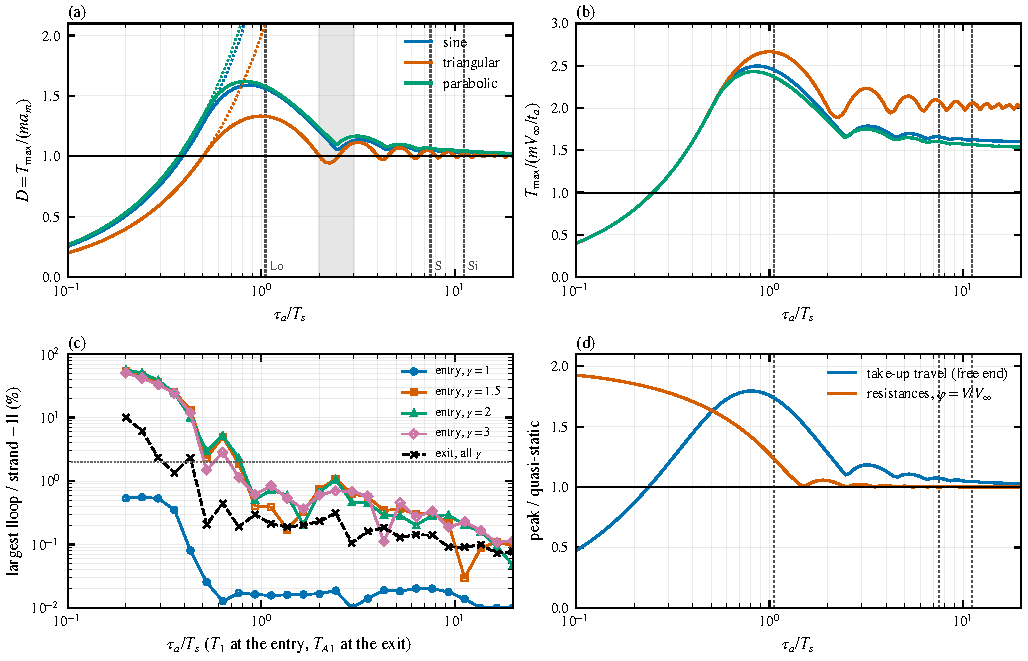
\includegraphics[width=\linewidth]{fig_startup}
  \caption{\TODO{fig\_startup caption (captions.md).}}
  \label{fig:startup}
\end{figure}
\begin{figure}[t]
  \centering
  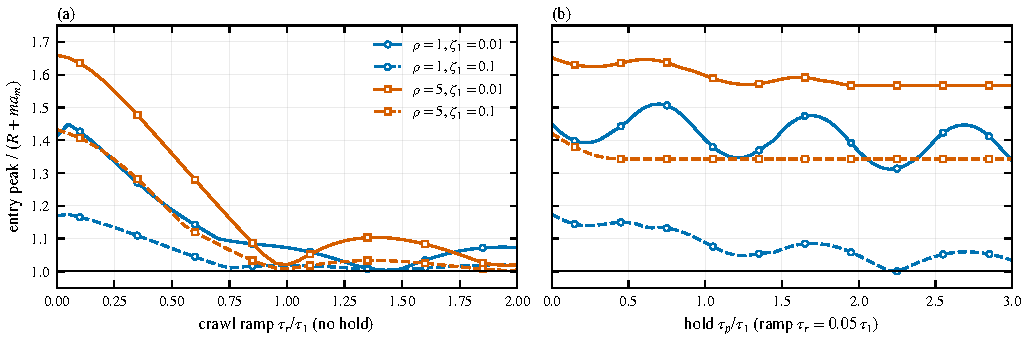
\includegraphics[width=\linewidth]{fig_crawl}
  \caption{\TODO{fig\_crawl caption (captions.md).}}
  \label{fig:crawl}
\end{figure}
% Wave law T = Z V exact for tau_a <= tau_s/2 (classic citation still to be
% found and read, 4.9 point 14); quasi-static limit; collapse of the loop;
% three formulas; fair comparison of profiles; rule tau_a >~ 2-3 tau_1;
% initial crawl (notes 4.17).
\TODO{Universal start-up curve.}

\subsection{Validity: slack, take-up and drive grip}\label{sec:validity}
\begin{figure}[t]
  \centering
  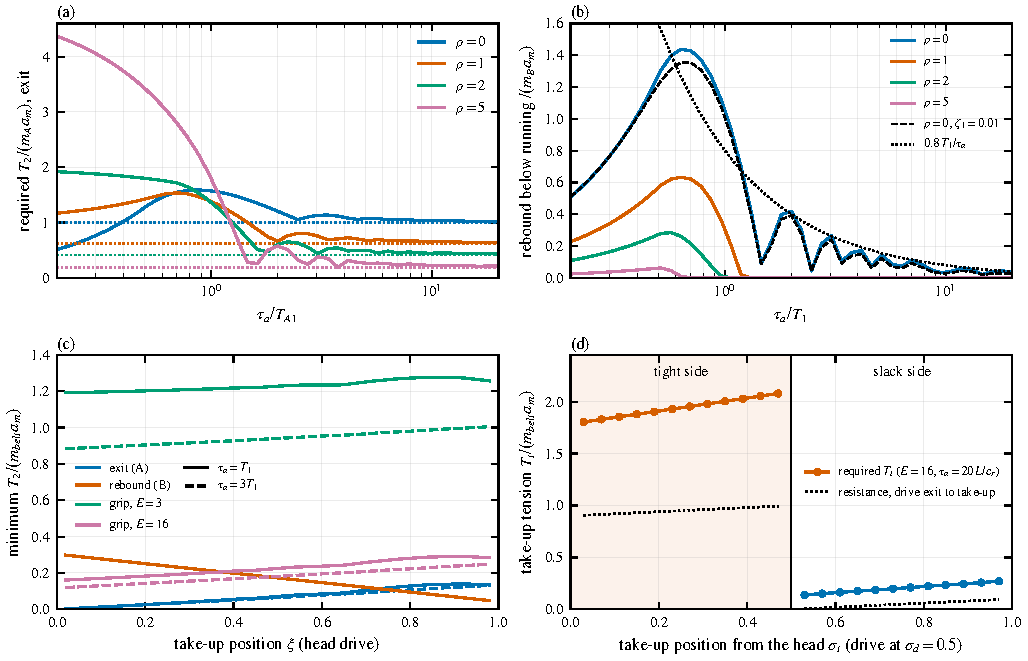
\includegraphics[width=\linewidth]{fig_validity}
  \caption{\TODO{fig\_validity caption (captions.md).}}
  \label{fig:validity}
\end{figure}
% Three conditions (notes 4.18); grip condition with the start factor from
% the universal curve; DIN 22101 sec. 7.3.1 and 8.2.2 (4.9 point 16).
\TODO{Validity conditions.}

% =====================================================================
% Section 6 -- Application to field conveyors. Written in step 6.6.
% Inputs: notes 4.26-4.27; fig_applications; table_applications (generated
% by maps/paper_tables.py). Lodewijks (1996) re-read in step 6.6: drive
% grip checked with the start-up factor 1.2 of a drain-type fluid coupling
% (Table 8.2, Eqs. 8.7-8.9, pp. 154-155); only single hinge elements, so no
% slip, at the drive pulleys (p. 137). DIN 22101 sec. 8.2.3 re-read: relative
% sag below 0.01 in steady operation, more allowed in non-steady operation.
% Numbers: paper_numbers.py, section "Application to field conveyors".
% Tests: test_applications.py, test_tables.py.
% =====================================================================
\section{Application to field conveyors}\label{sec:application}

\begin{figure}[tbp]
  \centering
  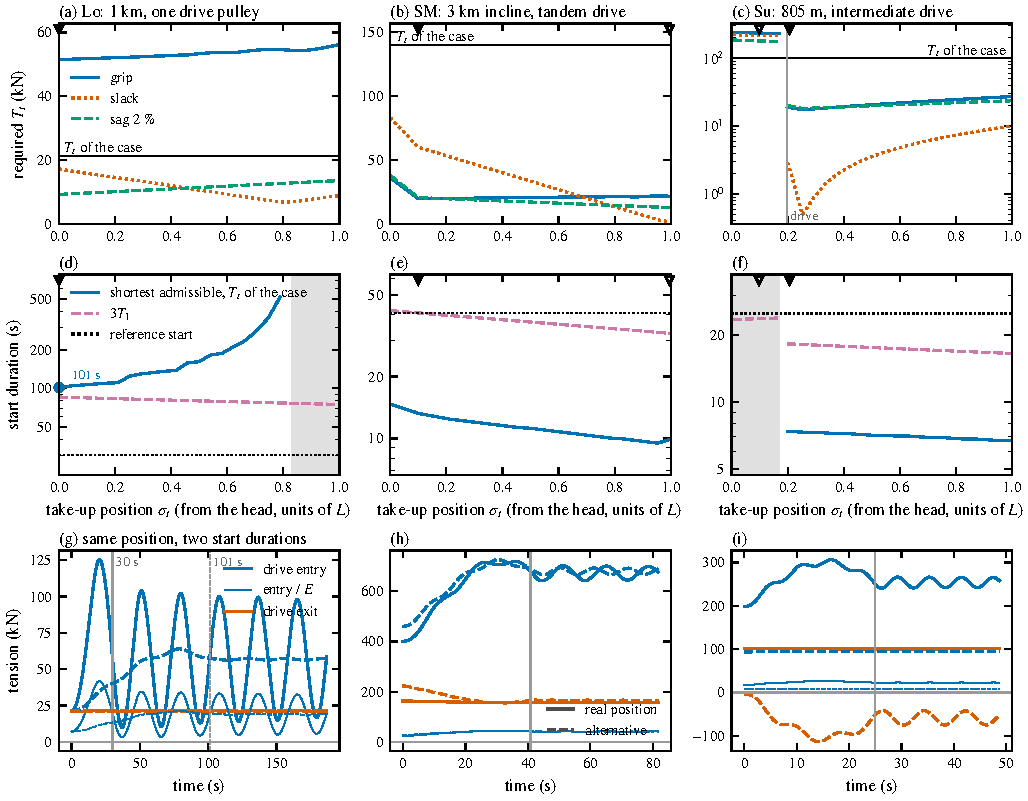
\includegraphics[width=\linewidth]{fig_applications}
  \caption{Start-ups of three conveyors from the literature in physical units, against the
  take-up position (sine profile, $\hat\zeta=0.01$, DIN~22101 strand resistances fitted to
  each $F_U$ and building up with the belt speed, gravity from each carry profile; the take-up
  is moved along the return strand with the case's counterweight). $\sigma_t$: take-up
  position from the head pulley along the return strand, in units of $L$ ($\sigma_t=\xi$ with
  a head drive). Filled triangle: real position; open triangle: alternative of the last row.
  Columns: Lo \citep{lodewijks1996}, \qty{1}{\kilo\metre}, one drive pulley
  ($\egrip=\NumLoGripFactor$), published \qty{30}{\second} start; SM
  \citep{suchorab2025longdistance}, \qty{3}{\kilo\metre} incline, tandem drive
  ($\egrip=16.4$), reference start $3\tper{1}=\qty{\NumSMReferenceStart}{\second}$ (assumed);
  Su \citep{surtees1995runback}, \qty{805}{\metre}, drive on the return strand at
  $\sigma_d=0.197$ ($\egrip=11.5$), published \qty{25}{\second} start. (a--c) Take-up tension
  required by each condition (positive tension along the loop during and after the start;
  grip; running sag below \qty{2}{\percent}), with the case's $\Tt$. (d--f) Shortest sine
  start that the case's $\Tt$ admits, with $3\tper{1}$ and the reference start; grey, no start
  is admissible (the running state already fails). (g) Lo at its real position: the published
  \qty{30}{\second} start (solid) and the shortest admissible one,
  \qty{\NumLoShortest}{\second} (dashed); grip is lost where the entry tension over $\egrip$
  (thin) exceeds the exit tension. (h) SM, real position (solid) and tail (dashed). (i) Su,
  real position (solid) and tight side of the drive (dashed), where the exit tension becomes
  negative. Values in \cref{tab:applications}.}
  \label{fig:applications}
\end{figure}
% Generated by maps/paper_tables.py (phase 5.6) from maps/applications.py; do not edit by hand.
\begin{table*}[t]
\centering
\footnotesize
\setlength{\tabcolsep}{3.5pt}
\begin{threeparttable}
\caption{Start-ups of three conveyors in physical units \citep[Lo, SM, Su:][]{lodewijks1996,suchorab2025longdistance,surtees1995runback}, real take-up position and an alternative (sine profile, $\hat\zeta=0.01$, DIN~22101 strand resistances fitted to $F_U$ and starting with the belt speed, gravity from the carry profile, the case's counterweight in every position). $\sigma_t$: take-up position from the head pulley along the return strand, in units of $L$. Peak drive-entry tension and its ratio to the running value; lowest drive-exit tension during and after the start; carriage travel; take-up tension required by the three conditions (positive tension along the loop, grip $T_\mathrm{entry}\le E\,T_\mathrm{exit}$, running sag below 2\,\%), the one that governs and the running exit tension it implies; shortest sine start that the case's $T_t$ admits.}
\label{tab:applications}
\begin{tabular}{@{}lrrrrrrrrrlrr@{}}
\toprule
 & & & & & \multicolumn{2}{c}{Entry peak} & Exit & & \multicolumn{3}{c}{Required} & Shortest \\
\cmidrule(lr){6-7}\cmidrule(lr){10-12}
Take-up & $\sigma_t$ & $t_1$ & $t_a$ & $t_a/t_1$ & (kN) & /running & min. & Travel & $T_t$ & governs & $T_2$ & start \\
 & & (s) & (s) & & & & (kN) & (m) & (kN) & & (kN) & (s) \\
\midrule
\multicolumn{13}{@{}l}{Lo: 1~km, one drive pulley ($\mathrm{e}^{\mu\theta}=3.0$), $T_t=21.3$~kN; published start 30~s} \\
real, 30~s & 0.001 & 28.5 & 30 & 1.05 & 125 & 2.21 & $21$ & 8.43 & 51.5 & grip & 51.5 & 101 \\
real, shortest start & 0.001 & 28.5 & 101 & 3.56 & 64 & 1.13 & $21$ & 3.20 & 21.3 & grip & 21.3 & 101 \\
tail, 30~s & 0.995 & 24.9 & 30 & 1.20 & 108 & 2.06 & $13$ & 5.15 & 56.1 & grip & 51.8 & -- \\
\midrule
\multicolumn{13}{@{}l}{SM: 3~km incline, tandem drive ($\mathrm{e}^{\mu\theta}=16.4$), $T_t=140$~kN; start $3t_1$ (assumed)} \\
real & 0.100 & 13.6 & 41 & 3.00 & 720 & 1.07 & $156$ & 0.96 & 60.0 & slack & 77.4 & 13 \\
tail & 0.995 & 10.8 & 41 & 3.77 & 726 & 1.07 & $155$ & 0.44 & 21.7 & grip & 46.9 & 10 \\
\midrule
\multicolumn{13}{@{}l}{Su: 805~m, drive at $\sigma_d=0.197$ ($\mathrm{e}^{\mu\theta}=11.5$), $T_t=100$~kN; published start 25~s} \\
real (after the drive) & 0.207 & 6.1 & 25 & 4.11 & 307 & 1.21 & $100$ & 0.25 & 19.8 & sag & 20.4 & 7 \\
tight side & 0.098 & 7.9 & 25 & 3.16 & 95 & 1.01 & $-114$ & 0.00 & 234.0 & grip & 75.2 & -- \\
\bottomrule
\end{tabular}
\begin{tablenotes}[flushleft]
\footnotesize
\item Slack: positive tension along the loop; in SM it is the weight of the return strand held from the take-up near the high end, at rest. Shortest start: --, none (the running state already fails with the case's $T_t$). The shortest start does not account for belt strength or motor torque. Su, tight side: the exit tension is negative already in running.
\end{tablenotes}
\end{threeparttable}
\end{table*}


The formulas of Section~\ref{sec:results} rest on idealised resistances and a horizontal
path. To see how the take-up position acts on real layouts, three conveyors of
\cref{tab:cases} are started in physical units with the full model: a \qty{1}{\kilo\metre}
conveyor with a single drive pulley and published speed-controlled starts
\citep[\S8.6.2]{lodewijks1996}, a \qty{3}{\kilo\metre} incline with a tandem head drive
\citep{suchorab2025longdistance}, and an \qty{805}{\metre} conveyor whose drive sits on the
return strand \citep{surtees1995runback}. Resistances follow DIN~22101 strand by strand, with
the coefficient fitted to the running peripheral force of each case, and build up with the
belt speed; gravity enters through each carry profile; the start is a sine profile with the
base damping $\hat\zeta=0.01$. The take-up is moved along the whole return strand with the
counterweight of the case, so $\Tt$ and $\beta$ stay fixed. At fixed take-up mass the total
tension is $\Tt$ plus a field that does not depend on $\Tt$, so each condition of
Section~\ref{sec:validity} gives a closed bound on $\Tt$ from a single run: positive tension
along the loop during and after the start, drive grip, and a running sag below
\qty{2}{\percent}. The last is the value used in the design calculations of
\citet{surtees1995runback}; DIN~22101 recommends less than \qty{1}{\percent} in steady
operation, mainly for energy efficiency \citep[\S8.2.3]{din22101}. The largest of the three
bounds is the required take-up tension, and the shortest admissible start is the shortest
sine start for which the case's $\Tt$ meets all three, at that duration and beyond. The
second condition, that the take-up follows the belt, never comes close: its margin is at
least \NumAppAccelMarginMin\ in all runs. Resizing the counterweight to keep the running exit
tension, instead of keeping the counterweight, changes the required tension and $\tper{1}$ by
less than \qty{0.3}{\percent}.
% tests: test_applications.py (exact superposition; slow-start limit equal to the running grip
% condition; carriage margin > 10; same-counterweight convention immaterial within 0.3 %)

\paragraph{One drive pulley: the grip sets the start time.} Lodewijks' conveyor has a single
drive pulley with $\egrip=\NumLoGripFactor$ and a take-up tension of
\qty{\NumLoTt}{\kilo\newton}, which he dimensioned for grip with the start-up factor 1.2 of a
drain-type fluid coupling \citep[Table~8.2 and Eqs.~8.7--8.9]{lodewijks1996}. His
\qty{30}{\second} speed-controlled starts last about one fundamental period and fall in the
overshoot of the universal curve: across the start profiles of his Table~8.7 the ratio of
drive-entry to drive-exit tension reaches \NumLoGripRatioMin\ to \NumLoGripRatioMax, against
the limit of \NumLoGripFactor. With the sine profile the belt would need
\qty{\NumLoTtReq}{\kilo\newton} at the take-up, \NumLoSineTtFactor\ times the installed
tension, to stay in grip. His simulations could not show this, since the drive pulleys were
modelled without slip \citep[p.~137]{lodewijks1996}. With his take-up the shortest admissible
sine start is \qty{\NumLoShortest}{\second}, \NumLoShortestOverPeriod\ periods, above the
$2$--$3\,\tper{1}$ of the design rule: with one drive pulley the grip, not the dynamic
amplification, fixes the start time. Moving the take-up away from the drive adds the
resistance of the return run to the required tension, while the required running exit
tension hardly changes (\cref{tab:applications}), and beyond $\xi=\NumLoXiLimit$ the installed
tension no longer holds grip even in steady running (\cref{fig:applications}a,~d). The real
position, next to the drive, is the best one.

\paragraph{Tandem drive on an incline: the statics decide.} The incline of
\citet{suchorab2025longdistance} has a tandem drive ($\egrip=16.4$) and a take-up tension of
\qty{\NumSMTt}{\kilo\newton}. Its take-up sits at $\xi=0.1$, near the high end, where at rest
it must hold the weight of the return strand down the slope: this alone requires
\qty{\NumSMTtReq}{\kilo\newton}, against \qty{\NumSMTtReqTail}{\kilo\newton} with the take-up
at the tail, where grip governs, and up to \qty{\NumSMTtReqMax}{\kilo\newton} next to the
drive. The installed tension covers every position, and the start could be as short as
\qty{\NumSMShortest}{\second}, about \NumSMShortestOverPeriod\ fundamental period. Moving the
take-up to the tail shortens the fundamental period by \qty{\NumSMPeriodChange}{\percent}
(\qty{\NumLoPeriodChange}{\percent} in Lodewijks' conveyor), but changes the peak drive-entry
tension by less than one per cent (\cref{tab:applications}): with a large wave-speed ratio
the carry strand dominates strand~B wherever the take-up is.

\paragraph{Drive on the return strand: the tight side.} Surtees' conveyor has its drive at
$\sigma_d=0.197$ from the head and the take-up right after it, on the slack side. There the
running sag governs and requires \qty{\NumSuTtReq}{\kilo\newton}, close to the lowest value
along the slack side (\qty{\NumSuTtReqBest}{\kilo\newton}); the installed
\qty{100}{\kilo\newton} admits starts from \qty{\NumSuShortest}{\second}, about
\NumSuShortestOverPeriod\ fundamental periods. On the tight side of the drive the take-up
would need \qty{\NumSuTtReqTight}{\kilo\newton}, \NumSuTightFactor\ times more: with the
installed counterweight the exit tension is negative already in running and falls to
\qty{\NumSuExitTight}{\kilo\newton} during the start (\cref{fig:applications}i). The
impractical region of Section~\ref{sec:validity} appears on a real layout.

\paragraph{What the take-up position does on real conveyors.} In these three conveyors the
take-up position acts mainly through the statics: through the resistance of the return run
between the drive and the take-up, and through the weight of the return strand on a slope.
Its dynamic effect, a fundamental period that changes by \NumLoPeriodChange\ to
\qty{\NumSMPeriodChange}{\percent} between the real position and the tail, enters through the
start time, which scales with $\tper{1}$. With one drive pulley the grip fixes the start time;
with a tandem drive or a generous take-up tension the three conditions admit starts of about
one fundamental period, and the limits then come from the belt strength and the motor, which
this analysis does not evaluate. In Lodewijks' and Surtees' conveyors the designers placed
the take-up at, or very near, its best position; in the incline the positions near the tail
would be the best and the one next to the drive the worst, and the installed counterweight
covers both.

% =====================================================================
% Section 7 -- Discussion. Written in step 6.7.
% Inputs: 4.9 points 6, 8, 10, 13 and 15; notes 4.27, 4.31 (correction:
% the take-up records that damp out in one or two cycles are those of
% kulinowski2013, Fig. 9, not harrison1983, whose Fig. 5e shows several
% slow cycles), 4.33 (remissions to Sections 5.3 and 6).
% Statements re-checked in the PDFs in step 6.7: nordell1984 (retarder of
% 6000 lb, 2720 kgf, in both directions), kulinowski2013 (slip on drum AB in
% all recorded starts; Fig. 9), kulinowski2021 (29-37 kN), kung2005henderson
% (counterweight pulled against the mechanical stops; low-tension wave from
% the take-up in stops without power; counterweight about 10 % over design),
% zamorano1991 (counterweight travel larger than the available travel
% damaged the tower), harrison1985b (buffer; take-up mass hit the
% structure when stopping). poe2000sheave, surtees1995runback and song2003
% as read in phases 3.7 and 4.4 (notes by source).
% Step 6.7b (Beltcon review): nordell1987 (p. 9: hydraulic retarder, damping
% towards a fixed take-up), morrison1987 (pp. 10-11: friction, inertia, fluid
% coupling), barfoot1997 (pp. 2-3), hou2008 (Sect. 3.1), checked in the PDFs.
% [HB1989] marks what to revisit with Harrison and Barfoot (1989).
% =====================================================================
\section{Discussion}\label{sec:discussion}

\subsection{Relation to practice and to previous models}\label{sec:relation}

\paragraph{The practice of take-up placement.} The results give a mechanical content to
the reasons of Section~\ref{sec:intro}. A take-up right after the drive keeps the tension
of the belt leaving the drive constant \citep{lodewijks2013} because strand~A, the only
belt between the drive exit and the free end, is then short: its dynamic tension during a
start is $D(t_a/\tper{A1})\,m_Aa_m$, with $m_A=\mu_r\xi L$, and vanishes as the take-up
approaches the drive (Eq.~\eqref{eq:startup_formulas}). Harrison's remedy of a take-up at
the tail \citep{harrison1985b} is consistent with the strand picture: the whole return
strand then becomes strand~A and is set in motion by the drive exit from the start, instead
of being reached by the stretching front only after it has gone round the carry strand and
the tail. The same picture accounts for the opposite concern of designers: with the take-up
at the tail of a long, low-lift conveyor, strand~A is the whole return strand, which the
take-up ``has to move \ldots\ in order to pull belt out of the drive area'', so the start
must be very long or the take-up tension high if the drive is not to slip
\citep{barfoot1997}. The fundamental period also falls when the take-up moves to the tail, by up to
a factor \NumHeadTailRatioGammaOne\ for equal wave speeds; in the conveyors of
Section~\ref{sec:application}, whose carry strands are two to three times slower than their
return strands, it falls by \NumLoPeriodChange\ and \qty{\NumSMPeriodChange}{\percent}
between the real position and the tail. In all three conveyors, however, the take-up position
acted mainly through the statics, through the resistance of the return run between the drive
and the take-up and through the weight of the return strand on a slope, and in two of the
three the real position was at or near the best one. Moving the
take-up is therefore a lever on the start time, which scales with $\tper{1}$, more than on
the peak tensions, which the start time controls (Section~\ref{sec:startup}). The other
reasons quoted in Section~\ref{sec:intro} lie outside the model: the horizontal curve of
ZISCO \citep{nordell1997zisco}, the second drive of \citet{kruse2019overland} and the drift
stop simulated by \citet{cdi2002}, in which the drive is not speed-controlled.
% [HB1989] Add the relation to Harrison and Barfoot (1989) here once read.

\paragraph{Previous continuum models.} The decoupling that \citet{song2012} obtained by
moving the take-up to the tail is the free end at one particular position; it holds at any
position, but the two strands are then the ones that the take-up position defines, and with
the take-up at the head, where their conveyor has it, the fundamental period is
\qty{\NumSongPeriodHeadLight}{\second} rather than \qty{\NumSongPeriodTailLight}{\second}.
The single-span formulation of \citet{pang2015} and \citet{li2018} is a different physical
model rather than a less accurate one. Their end mass moves with the belt and therefore
shares the rigid-body acceleration of the start, as a cage at the end of a hoisting rope
would; a take-up pulley is not moved by a uniform translation of the belt along its path
(Section~\ref{sec:increment}). The two models share the characteristic equation of a tail
take-up on a uniform loop, but not the response: with a pulley, the start does not excite
the family $\Omega\tan\Omega=2/\beta$ at all, and the response to the drive acceleration
does not depend on the take-up mass (Section~\ref{sec:frequencies}). For a gravity take-up
the mass ratio is tied to the take-up tension by Eq.~\eqref{eq:beta_tension}, so a change of
counterweight at fixed rigging, as in the study of \citet{gao2026}, changes the pre-tension
as well. In their conveyor the inertia alone would change the fundamental period by
\qty{\NumShiftG}{\percent}; the effects they report most likely come from the change of
static tension.

\paragraph{Drive grip.} The grip condition of Section~\ref{sec:validity} is not new; what
the universal curve adds is the start-up factor, which follows from the start time relative
to the fundamental period instead of being fixed in advance. It matters most with a single
drive pulley. Lodewijks' speed-controlled starts of \qty{30}{\second} would have needed the
belt to grip with a tension ratio of \NumLoGripRatioMin\ to \NumLoGripRatioMax\ against a limit of
\NumLoGripFactor, a slip that his model, built without slip at the drive pulleys, could not
show (Section~\ref{sec:application}). Slip at the drive is observed in the field:
\citet{kulinowski2013} report it on one drive drum during all the recorded starts of a mine
conveyor with fluid couplings, and \citet{kulinowski2021} during a start with a non-typical
sequence of motors. Checking grip through the start, and not only in steady running, is
therefore part of choosing the start time.

\paragraph{Devices that resist the carriage.} Equation~\eqref{eq:transmission_z} extends the
free end to any take-up whose belt-side impedance $z_t$ is known: a front is transmitted with
the fraction $z_t/(z_t+2Z_r)$. A hydraulic buffer under the carriage, as in the modified
design of \citet{harrison1985b}, transmits part of every front at once; a rigid end stop
($z_t\to\infty$) turns the take-up into a fixed pulley around which the belt runs, with the
spectrum $(\mat B\mat A)_{12}=0$ of Section~\ref{sec:eigen}; and a motion retarder, such as
the hydraulic retarder of \citet{nordell1984}, represented in their model by a drag of
2720~kgf in both directions, keeps the carriage locked, and the take-up transparent, until
the drag is exceeded; the belt beyond their take-up followed the drives for about a second
and then came free (Section~\ref{sec:fieldchecks}). Nordell observed that adding damping to
that retarder raised the shock force ``toward the characteristics of a fixed take-up''
\citep{nordell1987}, and \citet{morrison1987} found both effects in finite-element
simulations: a front passed the take-up while friction held the counterweight, was almost
totally reflected once it moved, and was still transmitted in small part through the inertia
of the counterweight. The free-end results of this
paper therefore hold while the carriage moves freely; each of these devices moves the
take-up towards the fixed pulley, and the impedance formula gives the size of the change for
the linear ones.

\subsection{Limitations}\label{sec:limitations}

\paragraph{Take-up.} The take-up is assumed to move without friction, with the inertia of
its pulley, ropes and sheaves neglected (A7). Measured carriage forces are less ideal. Sheave
friction raised the force on a take-up carriage by up to \qty{26}{\percent} above the
counterweight, with hysteresis between stretch and recovery \citep{poe2000sheave}, and the
take-up force of a mine conveyor fluctuated between \num{29} and \qty{37}{\kilo\newton}
because of the inertia of the weights and the efficiency of the tensioning system
\citep{kulinowski2021}. Measured carriage displacements also die out within one or two cycles
after a start \citep[Fig.~9]{kulinowski2013}, faster than the Kelvin--Voigt damping of the
belt alone would allow, although the take-up record of \citet[Fig.~5e]{harrison1983} shows
several slow cycles. Friction of this kind makes the take-up partly transparent while the
carriage sticks (Section~\ref{sec:relation}) and damps the slow modes. It changes neither
the peak tensions of a speed-controlled start, which depend little on damping
(Section~\ref{sec:startup}), nor the free-end limit while the carriage slides, but it
affects the oscillations after the start, for which the undamped rebound of
Section~\ref{sec:validity} is an upper bound. The carriage travel is also limited. Field
reports describe a counterweight jammed in its tower, which left an incline without
slack-side tension and let it run back \citep{surtees1995runback},
counterweights pulled against their end stops \citep{kung2005henderson,song2003} and a tower
damaged during a full-load start because the counterweight travel exceeded the travel
available \citep{zamorano1991}. The take-up travel formula of Eq.~\eqref{eq:startup_formulas}
and the velocity bounds of Section~\ref{sec:validity} size the travel and speed that the
tower must allow; contact with a stop lies outside the linear model.

\paragraph{Belt.} The belt is linear and Kelvin--Voigt. At low tension the sag between
idlers stiffens the belt and slows the waves \citep{ellis1987}; the slack condition of
Section~\ref{sec:validity} marks where the total tension approaches zero and this assumption
fails. The modulus of textile belts also depends on tension and temperature: it falls by
\qtyrange{13}{30}{\percent} at low load and by \qtyrange{8}{18}{\percent} at
\qty{50}{\degreeCelsius} \citep{zarzycki2023}, and the wave speed measured on samples of a
fabric and a steel-cord belt rises with tension, steeply at low tension \citep{hou2008},
which changes the wave speeds and,
through them, every period in seconds, but not the dimensionless results. Damping
proportional to stiffness is a modelling convenience that keeps the modes uncoupled, not a
measured law.

\paragraph{Resistances and drive.} The motion resistances are a load that appears along the
whole loop at once, with an onset that follows the drive speed. In a real start they appear
behind the stretching front and depend on the local belt speed, so the step onset of
Section~\ref{sec:startup} is an upper bound. The drive imposes the belt velocity, which
represents speed-controlled drives (Section~\ref{sec:torque}). Drives without speed control,
such as fluid couplings or wound-rotor motors started in steps, change the spectrum, as the
case of Harrison's conveyor shows (Section~\ref{sec:fieldchecks}), and need not reflect the
waves that reach them: in simulations, a drive on a fluid coupling at low fill let most of a
returning front pass \citep{morrison1987}. Stops without power,
in which the drive is free and the take-up itself can launch a low-tension wave
\citep{kung2005henderson}, are not analysed. The shortest admissible starts of
Section~\ref{sec:application} do not check belt strength or motor torque.

\paragraph{Layout.} The model has one drive station, homogeneous strands, a straight path in
plan and the take-up on the return strand. Distributed drives, horizontal curves, loading
over part of the carry strand and a take-up on the carry strand are outside it, although the
transfer-matrix formulation extends to more segments and the code accepts a take-up at any
point of the loop.

\paragraph{Validation.} The verification is complete within the idealisation, but the field
checks are partial (Section~\ref{sec:validation}). A start record that combines a free
gravity take-up, a speed-controlled drive, a time history of the take-up and published
conveyor parameters would test the model directly. Modern overland conveyors already record
the take-up position in operation \citep{kruse2019overland}; publishing such a record with
the conveyor data would close this gap.

% =====================================================================
% Section 8 -- Conclusions. Step 6.7.
% =====================================================================
\section{Conclusions}\label{sec:conclusions}
\TODO{Conclusions: one paragraph per contribution, with the numbers that
support it (macros from paper\_numbers.tex).}

% =====================================================================
% Back matter required by the target journals (check in phase 7).
% =====================================================================
\section*{Data availability}
\TODO{Code and data: beltloop, https://github.com/daniel-gonzalezm/beltloop;
archived version with DOI on Zenodo and MIT licence at submission. All
figures, tables and numbers of the paper are produced by the scripts in
maps/ and validation/.}

\section*{Declaration of competing interest}
\TODO{Statement.}

\section*{Funding}
\TODO{Statement (for example: no specific grant).}

\section*{Declaration of generative AI and AI-assisted technologies in the manuscript preparation process}
% Elsevier requires this statement when such tools were used; Springer
% and Wiley have their own policies. Wording to be written by the author
% in phase 7, following the policy of the chosen journal.
\TODO{Statement, if applicable.}

\section*{Acknowledgements}
\TODO{Acknowledgements, if any.}


\bibliographystyle{plainnat}   % elsarticle-num (or the journal style) in phase 7
\bibliography{references}

\appendix
% Appendix A -- transfer matrices and orthogonality (model.tex, step 6.3).
\section{Transfer matrices and orthogonality}\label{app:transfer}

\paragraph{Matrices of the two strands.} With $\mat S_r(\ell)=\mat S(\ell,\Omega)$ and
$\mat S_c(\ell)=\mat S(\ell,\gamma\Omega)$, and positions in units of $L$, the products
of~\eqref{eq:chareq} are those of \cref{tab:AB}; the factors are written from right
to left in the order in which the belt meets the segments. A take-up on the tight side
of an intermediate drive belongs to the same family as one on the slack side: reversing
the direction of travel exchanges the two.

\begin{table}[h]
  \centering
  \caption{Transfer matrices of strand~A, from the drive exit to the take-up, and of
  strand~B, from the take-up to the drive entry, with the take-up on the return
  strand.}
  \label{tab:AB}
  \small
  \begin{tabular}{@{}lll@{}}
    \toprule
    Drive position & $\mat A$ & $\mat B$\\
    \midrule
    Head ($\sigma_d=0$) & $\mat S_r(\sigma_t)$ & $\mat S_c(1)\,\mat S_r(1-\sigma_t)$\\
    Return strand, take-up downstream ($\sigma_d<\sigma_t$) & $\mat S_r(\sigma_t-\sigma_d)$
      & $\mat S_r(\sigma_d)\,\mat S_c(1)\,\mat S_r(1-\sigma_t)$\\
    Return strand, take-up upstream ($\sigma_t<\sigma_d$)
      & $\mat S_r(\sigma_t)\,\mat S_c(1)\,\mat S_r(1-\sigma_d)$ & $\mat S_r(\sigma_d-\sigma_t)$\\
    Tail ($\sigma_d=1$) & $\mat S_r(\sigma_t)\,\mat S_c(1)$ & $\mat S_r(1-\sigma_t)$\\
    \bottomrule
  \end{tabular}
\end{table}

\paragraph{Direction of travel.} Let $\mat Q=\operatorname{diag}(1,-1)$. Each factor
$\mat E\in\{\mat S,\mat J\}$ satisfies $\mat Q\mat E\mat Q=\mat E^{-1}$, so the product
$\mat P=\mat E_m\cdots\mat E_1$ of a chain and the product $\mat P^{\mathrm R}=\mat E_1\cdots\mat E_m$
of the reversed chain are related by $\mat P^{\mathrm R}=\mat Q\mat P^{-1}\mat Q$. Since
$\det\mat P=1$, $(\mat P^{-1})_{12}=-P_{12}$ and $P^{\mathrm R}_{12}=P_{12}$: the condition
$P_{12}=0$, and with it the spectrum, does not depend on the direction of travel. The
same relation gives $\operatorname{tr}\mat P^{\mathrm R}=\operatorname{tr}\mat P$, so the
torque-controlled equation~\eqref{eq:chareq_torque} is also invariant.

\paragraph{Orthogonality.} For two modes $(W_i,Y_i)$ and $(W_j,Y_j)$, multiplying
\eqref{eq:eigen} for mode $i$ by $W_j$, integrating over the segments and integrating by
parts gives
\begin{equation}\label{eq:orth_derivation}
  \Omega_i^2\int_0^2\hat\mu\,W_iW_j\,\dd x=\int_0^2W_i'W_j'\,\dd x
  -W_i'(\xi)\bigl[W_j(\xi^-)-W_j(\xi^+)\bigr],
\end{equation}
because $W_j$ vanishes at the drive and $W$ and $W'$ are continuous at the head and
tail pulleys. At the take-up $W_i'$ is continuous and, by~\eqref{eq:eigen_tu},
$W_j(\xi^-)-W_j(\xi^+)=2Y_j$ and $W_i'(\xi)=\tfrac12\beta\Omega_i^2Y_i$, so the boundary term is
$\beta\Omega_i^2Y_iY_j$ and
\begin{equation}\label{eq:orth}
  \Omega_i^2\left(\int_0^2\hat\mu\,W_iW_j\,\dd x+\beta\,Y_iY_j\right)=\int_0^2W_i'W_j'\,\dd x .
\end{equation}
The right-hand side is symmetric in $i$ and $j$; subtracting the same identity with $i$
and $j$ exchanged shows that modes with distinct frequencies are orthogonal with
respect to~\eqref{eq:inner}, and then~\eqref{eq:orth} gives
$\int_0^2W_i'W_j'\,\dd x=\Omega_i^2m_i\delta_{ij}$. The modal equations~\eqref{eq:modal}
follow by projecting~\eqref{eq:pde_nd}--\eqref{eq:bc_nd} on $(W_k,Y_k)$ with the same
inner product: the inertial and resistance loads act on the belt only, which is why
$\Gamma_k$ and $R_k$ carry no take-up term.

% =====================================================================
% Appendix B -- Numerical methods (notes 4.8 and 4.9 point 5). Written in
% step 6.4. Implementation: beltloop/src/beltloop (eigen.py, transfer.py,
% forcing.py, response.py, lumped.py); numbers in paper_numbers.tex
% (section "Appendix B").
% =====================================================================
\section{Numerical methods}\label{app:numerics}

The closed-form solution is implemented in the open-source Python package
\texttt{beltloop} (see Data availability), together with the lumped-mass model of
Section~\ref{sec:lumped} and the scripts that produce every figure, table and number
of the paper. This appendix describes the numerical steps that the closed form leaves
open, and the lumped-mass model used for its verification.

\paragraph{Natural frequencies.} The roots of~\eqref{eq:chareq} are found without a
search grid, from the interlacing property of Section~\ref{sec:properties}. The poles
of~\eqref{eq:receptance}, the fixed--free frequencies of each strand, are bracketed
first with the scaled Pr\"ufer angle $\phi=\operatorname{atan2}(\kappa W,W')$ of the
chain started from $(W,W')=(0,1)$ at the drive. Inside a segment $\phi$ grows by
$\kappa\ell$; at a change of density $W$ and $W'$ are continuous, so $\tan\phi$ is
multiplied by the ratio of the wavenumbers and $\phi$ is mapped within its quadrant.
The end value $\phi(\Omega)$ increases with $\Omega$ (Sturm), and the $j$-th
fixed--free frequency is the root of $\phi(\Omega)=(j-\tfrac12)\pi$. Since each of the
$m$ density changes of a strand moves $\phi$ by less than $\pi/2$, that root lies in
\begin{equation}\label{eq:prufer_bracket}
  \frac{(j-\tfrac12)\pi-\tfrac{m}{2}\pi}{\Phi}\le\Omega_j\le\frac{(j-\tfrac12)\pi+\tfrac{m}{2}\pi}{\Phi},
  \qquad \Phi=\sum_i\kappa_i\ell_i/\Omega,
\end{equation}
which is used as the bracket for Brent's method. The poles of the two strands are then
merged and sorted, $p_1\le p_2\le\dots$, and the $k$-th natural frequency is sought in
$(p_{k-1},p_k)$, $p_0=0$. In that interval $D/(\beta\Omega^2A_{22}B_{11})$ increases
from $-\infty$ to $+\infty$ and $A_{22}B_{11}$ keeps its sign, so $D$ multiplied by that
sign changes from negative to positive across the interval; the end values are replaced
by these limit signs, and Brent's method converges to the single root. A pair of
coincident poles is itself a root and is returned exactly. The method finds every
root, including pairs separated by $O(\beta)$ near nearly coincident poles, which a grid
search with a fixed step misses when $\beta$ is small. The limit $\beta=0$ returns the
poles themselves. For the drive without speed control, Eq.~\eqref{eq:chareq_torque},
the interlacing argument is not available: real roots are located by a sign scan on a
fine grid, and the complex roots with a slip dashpot by Newton's method started from
the root with prescribed velocity, the limit $\hat c\to\infty$. Both serve only for the
checks of Section~\ref{sec:fieldchecks}.
% tests: test_eigen.py (fixed-free roots, all roots against a dense scan, close roots
%        at beta = 1e-7, FE agreement, torque variant), test_harrison.py (damped drive)

\paragraph{Modes and modal quantities.} Each mode is obtained by propagating
$(W,W')=(0,1)$ through the chain with the matrices~\eqref{eq:transfer}, with the jump of
$W$ and the take-up amplitude $Y$ of~\eqref{eq:eigen_tu} at the take-up. On a segment
$W$ is a combination of $\cos\kappa x$ and $\sin\kappa x$, so the integrals that enter
the modal mass~\eqref{eq:inner}, the participation factors~\eqref{eq:participation}
and the stiffness identity $\int W'^2\dd x=\Omega^2m$ are evaluated in closed form,
segment by segment; the last identity is kept as a check of every mode. The modes are
normalised to unit modal mass. The take-up term $\beta Y^2$ of the modal mass requires
$\beta>0$; the limit $\beta\to0$ of the forced response is computed with a small
$\beta$, which the free-end structure makes harmless.
% tests: test_modes.py (interfaces, closed-form integrals, weighted orthogonality,
%        Parseval, quasi-static sums)

\paragraph{Exact integration of the modal equations.} On each interval of a start-up
profile the loads $\hat a(\tau)$ and $\varphi(\tau)$ are outputs of a small linear
system $\mat z'=\mat E\mat z$: the polynomial pieces of the triangular, parabolic and
piecewise-linear profiles, and the sine and cosine of the sinusoidal profile, whose
velocity gives the onset $\varphi=V/V_\infty$. Appending $\mat z$ to the state
$(p_k,p_k')$ of each mode gives an autonomous linear system, which is advanced exactly
to every output time by its matrix exponential, interval by interval, with the modal
state carried across the breaks. The integration has no time step and no truncation
error; it holds for any damping, including overdamped high modes, and for exact
resonance $\Omega_k=\varpi$. A jump of the drive velocity, as in the offset start of
\citet{lodewijks1996}, is replaced by a short ramp so that the load stays bounded.
% tests: test_response.py (exosystem against closed form, exact integration against an
%        ODE solver, residual amplitude at exact resonance, damping ratio)

\paragraph{Quasi-static split.} The modal sum~\eqref{eq:outputs} for the tension
converges slowly, because the tension is the derivative of the displacement and the
loads reach every mode. It is therefore split into the quasi-static
field~\eqref{eq:quasistatic}, summed in closed form, and a dynamic remainder. With
Kelvin--Voigt damping the quasi-static tension is exact but the strain lags; the
quasi-static modal coordinates are accordingly
$p_k^{\mathrm{qs}}=-(\Gamma_k\hat a_f+R_k\varphi_f)/\Omega_k^2$, where the lagged loads
obey $2\hat\zeta\hat a_f'+\hat a_f=\hat a$ and $2\hat\zeta\varphi_f'+\varphi_f=\varphi$,
a first-order filter with the same time constant for every mode, and
\begin{equation}\label{eq:split}
  \hat T=\hat T_{\mathrm{qs}}+\sum_k\left(q_k+2\hat\zeta q_k'\right)W_k',\qquad
  \hat y=\tfrac12\bigl(\hat a_fI_\mu+\varphi_fI_r\bigr)+\sum_kq_kY_k,\qquad
  q_k=p_k-p_k^{\mathrm{qs}},
\end{equation}
with $I_\mu=\int_0^2\int_\xi^x\hat\mu\,\dd x'\,\dd x$ and $I_r$ defined likewise. The
remainder $q_k$ is driven only by the rate of change of the quasi-static response and
converges fast with or without damping. With \NumSplitModes\ modes the tension differs
from a reference with \NumSplitRefModes\ modes by at most \num{\NumSplitErr} of its
maximum for $0\le\hat\zeta\le0.1$, against \num{\NumPlainErr} for the plain sum with the
same modes. Splitting off the undamped quasi-static response instead, $p_k-F_k/\Omega_k^2$,
leaves a remainder of order $2\hat\zeta F_k'/\Omega_k^2$, which converges as slowly as
the plain sum.
% tests: test_response.py (split convergence with damping, lagged loads, quasi-static
%        limit); numbers: paper_numbers.py, section "Appendix B"

\paragraph{Lumped-mass model.} The model of Section~\ref{sec:lumped} divides the loop,
from the drive exit to the drive entry, into $N$ elements with nodes at the head and
tail pulleys and at the take-up. Each element carries half of its mass at each end, a
linear spring $EA/h$ and a Kelvin--Voigt dashpot, so that the damping matrix is
$\mat C=t_v\mat K$. The take-up adds the carriage displacement $y_c$ as a degree of
freedom, with mass $\Mtu$ and the static force $\nstr\Tt$, and enters the element that
wraps the take-up pulley through its elongation $u_R-u_L+\nstr y_c$. The weight
components of belt and material along the path and the counterweight are constant
loads, the motion resistances are applied with the same onset $\varphi$ as in the
modal solution, and the two end nodes follow the prescribed drive displacement. The
static state is solved first, and the start is integrated with the Newmark
average-acceleration scheme, which is implicit, unconditionally stable, second-order
accurate and free of numerical damping; the time step is refined in proportion to the
element length, so that the convergence of \cref{fig:validation}(d) measures the
combined error in space and time.
% src/beltloop/lumped.py; tests: test_lumped.py, test_strands.py

% % Appendix C -- notes on the cases (if the table notes are moved out of
% Table tab:cases; decide in 6.8 or phase 7).
\section{Parameters of the field conveyors}\label{app:cases}
\TODO{Per-case notes and conventions (notes 4.21), only if they leave the table.}
  % step 6.8: empty; the case notes stay in Table 2 (decide in phase 7 if the table must shrink)

\end{document}
